\documentclass[mat1]{fmfdelo}
% \documentclass[fin1]{fmfdelo}
% \documentclass[isrm1]{fmfdelo}
% \documentclass[mat2]{fmfdelo}
% \documentclass[fin2]{fmfdelo}
% \documentclass[isrm2]{fmfdelo}

% naslednje ukaze ustrezno napolnite
\avtor{Tjaša Vrhovnik}

\naslov{Fareyevo zaporedje in Riemannova hipoteza}
\title{The Farey Sequence and The Riemann Hypothesis}

% navedite ime mentorja s polnim nazivom: doc.~dr.~Ime Priimek,
% izr.~prof.~dr.~Ime Priimek, prof.~dr.~Ime Priimek
% uporabite le tisti ukaz/ukaze, ki je/so za vas ustrezni
\mentor{izr.~prof.~dr.~Aleš Vavpetič}
% \mentorica{}
% \somentor{}
% \somentorica{}
% \mentorja{}{}
% \mentorici{}{}

\letnica{2019} % leto diplome

%  V povzetku na kratko opišite vsebinske rezultate dela. Sem ne sodi razlaga organizacije dela --
%  v katerem poglavju/razdelku je kaj, pač pa le opis vsebine.
\povzetek{V delu je predstavljeno Fareyevo zaporedje, njegova motivacija in lastnosti. Navedena je rekurzivna formula za izračun dolžine zaporedja $n$-tega reda in njeno asimptotično obnašanje. Izkaže se, da je Fareyevo zaporedje v bijekciji z množico Fordovih krogov. Razložen je geometrijski pomen lastnosti mediante in Fareyevih sosedov ter opisana konstrukcija vseh Fordovih sosedov danega Fordovega kroga. Definirane so Fordove krogle. S pomočjo delovanja grupe M\"obiusovih transformacij na množico Fordovih krogov je dokazana lastnost mediante. Predstavljena je Riemannova hipoteza in dve njeni ekvivalentni formulaciji. Dokazan je izrek, ki Fareyevo zaporedje preko Mertensove funkcije poveže z Riemannovo hipotezo.}

%  Prevod slovenskega povzetka v angleščino.
\abstract{The work presents the Farey sequence, its motivation and properties. A recursive formula for calculating the length of the sequence of order $n$ and its asymptotic behaviour are stated. The Farey sequence is in bijection with the set of Ford circles, therefore a geometric meaning of the mediant and the neighbours property is explained as well as the construction of all Ford neighbours to a given Ford circle. Moreover, Ford spheres are defined. Using the fact that the group of M\"obius transformations acts on the set of Ford circles, the mediant property for Ford circles is proved. Additionally, the Riemann hypothesis and two of its equivalent statements are presented. A theorem, connecting the Farey sequence, the Mertens function and the Riemann hypothesis, is proved.}

% navedite vsaj eno klasifikacijsko oznako --
% dostopne so na www.ams.org/mathscinet/msc/msc2010.html
\klasifikacija{11B57, 11M26, 51N20}
\kljucnebesede{Fareyevo zaporedje, Fordov krog, zeta funkcija, Riemannova hipoteza} % navedite nekaj ključnih pojmov, ki nastopajo v delu
\keywords{Farey sequence, Ford circle, zeta function, Riemann hypothesis} % angleški prevod ključnih besed

\zapisiMetaPodatke  % poskrbi za metapodatke in veljaven PDF/A-1b standard

% aktivirajte pakete, ki jih potrebujete
% \usepackage{tikz}
\usepackage{graphicx}

% za številske množice uporabite naslednje simbole
\newcommand{\R}{\mathbb R}
\newcommand{\N}{\mathbb N}
\newcommand{\Z}{\mathbb Z}
\newcommand{\C}{\mathbb C}
\newcommand{\Q}{\mathbb Q}

% matematične operatorje deklarirajte kot take, da jih bo Latex pravilno stavil
% \DeclareMathOperator{\conv}{conv}
\DeclareMathOperator{\re}{Re}

% vstavite svoje definicije ...
%  \newcommand{}{}

\begin{document}

%%%%%%%%%%%%%%%%%%%%%%%%%%%%%%%%%%%%%%%%%%%%%%%%%%%%%%%%%%%%%%%%%%%%%%%%%%%%%%%%%%%%%%%%%%%%%%%%%%%%%%%%%%%%%%%%%%%%%%%%%%%%%%%%%%%%%%%%%%%%%%%%%%
%
\section{Uvod}

Zgodovina Fareyevega zaporedja sega v London 18.~stoletja. Med letoma 1704 in 1841 je izhajal letni zbornik \emph{The Ladies Diary: or, the Woman's Almanack}, ki je povezoval ljubitelje matematičnih ugank. Bralce so namreč nagovarjali k pošiljanju in reševanju aritmetičnih problemov, ki so bili v zborniku objavljeni. Leta~1747 se je pojavilo naslednje vprašanje: Najti je potrebno število ulomkov različnih vrednosti, večjih od $0$ in manjših od $1$, katerih imenovalec je manjši od $100$. Odziv je bil precejšen, saj so se z iskanjem rešitve ukvarjali tako javnost kot pomembni matematiki tiste dobe. To je vodilo v razvoj Fareyevega zaporedja, ki ima nekaj presenetljivih lastnosti in uporabo na različnih področjih matematike.

Delo diplomskega seminarja je sestavljeno iz treh večjih enot. V prvi bomo predstavili zgodovinski pregled, definicijo, lastnosti in ocenili dolžino Fareyevega zaporedja. V drugem razdelku se bomo posvetili njeni geometrijski interpretaciji -- Fordovim krogom -- in opazili, da imata dve najpomembnejši lastnosti Fareyevega zaporedja tudi geometrijski pomen. Konstruirali bomo vse Fordove sosede danega Fordovega kroga. Navedli bomo možno posplošitev Fordovih krogov in definirali Fordove krogle. Ogledali si bomo predstavitev Fordovih krogov z uporabo algebre in kompleksne analize -- dokazali bomo, da grupa M\"obiusovih transformacij deluje na množico Fordovih krogov, od koder bo sledila že znana lastnost mediante. V zadnjem delu bomo obravnavali znamenit matematični problem, Riemannovo hipotezo. Predstavili bomo njeno motivacijo in navedli dve ekvivalentni formulaciji te domneve. Dokazali bomo povezavo Riemannove hipoteze s Fareyevim zaporedjem, pred tem pa se bomo seznanili s pojmi kot so Eulerjev produkt, Riemannova zeta funkcija, Bernoullijeva števila in polinomi, ter M\"obiusova in Mertensova funkcija.

Vse slike, pri katerih ni naveden vir, so avtorske; izdelane so s pomočjo programov GeoGebra in Octave.

%%%%%%%%%%%%%%%%%%%%%%%%%%%%%%%%%%%%%%%%%%%%%%%%%%%%%%%%%%%%%%%%%%%%%%%%%%%%%%%%%%%%%%%%%%%%%%%%%%%%%%%%%%%%%%%%%%%%%%%%%%%%%%%%%%%%%%%%%%%%%%%%%%
%
\section{Fareyevo zaporedje}

%%%%%%%%%%%%%%%%%%%%%%%%%%%%%%%%%%%%%%%%%%%%%%%%%%%%%%%%%%%%%%%%%%%%%%%%%
%
\subsection{Zgodovina Fareyevega zaporedja}

Vrnimo se k v uvodu omenjeni nalogi o številu ulomkov različnih vrednosti, manjših od $1$, z imenovalci manjšimi od $100$. Prvi odgovor na članek je bila tabela ulomkov z imenovalci manjšimi od $10$, nato pa še dve tabeli z rezultatoma $3055$ in $4851$. Leta 1751 je R.~Flitcon objavil pravilni odgovor $3003$, kateremu je dodal tudi opis postopka. Preden ga razložimo, si oglejmo Eulerjevo funkcijo in njene lastnosti, ki nas bodo pripeljale do rešitve. 
%
% Eulerjeva funkcija

\begin{definicija}
Preslikava \( \varphi \colon \mathbb{N} \rightarrow \mathbb{N}\), ki za vsako naravno število $n \geq 2$ prešteje števila, manjša od $n$, ki so $n$ tuja, za $n=1$ pa predpišemo $\varphi(1) = 1$, se imenuje \emph{Eulerjeva funkcija} $\varphi$.
\end{definicija}

\begin{primer}
Izračunajmo nekaj vrednosti Eulerjeve funkcije:

\( \varphi(1) = 1, \)

\( \varphi(2) = 1, \)

\( \varphi(3) = 2, \)

\( \varphi(4) = 2, \)

\( \varphi(8) = 4, \)

\( \varphi(9) = 6. \)

Opazimo, da za praštevilo $p$ velja $\varphi(p) = p-1.$
\end{primer}

\begin{trditev}
\label{trd:MultipEuler}
Če sta $k$ in $l$ tuji si števili, velja $\varphi (kl) = \varphi (k) \varphi (l)$, torej je Eulerjeva funkcija multiplikativna.
\end{trditev}

\begin{dokaz}
V dokazu multiplikativnosti si bomo pomagali z lastnostmi grup. 
Naj $\mathbb{Z}_{k}^\ast $ označuje grupo vseh obrnljivih elementov grupe $\mathbb{Z}_{k}$. Vemo, da so obrnljivi elementi grupe $\mathbb{Z}_{k}$ tista števila iz množice \( \{0, 1, \ldots, k-1 \}, \) ki so tuja $k$, zato je $|\mathbb{Z}_{k}^\ast| = \varphi(k).$  
Dobimo zvezi
\begin{align*}
|\mathbb{Z}_{kl}^\ast| &= \varphi(kl), \\
|\mathbb{Z}_{k}^\ast| |\mathbb{Z}_{l}^\ast| &= \varphi(k) \varphi(l).
\end{align*}
Znano je, da je preslikava \( \psi \colon \mathbb{Z}_{kl}^\ast \rightarrow \mathbb{Z}_{k}^\ast \times \mathbb{Z}_{l}^\ast \) za tuji naravni števili $k$ in $l$ izomorfizem grup. Ker je moč kartezičnega produkta dveh množic enaka produktu njunih moči, sledi 
\[ \varphi(kl) = |\mathbb{Z}_{kl}^\ast| = |\mathbb{Z}_{k}^\ast| |\mathbb{Z}_{l}^\ast| = \varphi(k) \varphi(l), \]
s čimer je multiplikativnost dokazana.
\end{dokaz}

\begin{trditev}
\label{trd:EulerPrastProd}
Vrednost Eulerjeve funkcije je enaka
\begin{equation}
\varphi(n) = n \prod_{p|n} \left (1 - \frac{1}{p} \right ),
\end{equation}
kjer so $p$ prafaktorji števila $n$.
\end{trditev}

\begin{dokaz}
Zapišimo $n$ kot produkt prafaktorjev, \(n=\prod_{i=1}^m p_i^{r_i}\), kjer so $r_i \in \mathbb{N}$ in $p_i$ različna praštevila.
Vrednost $\varphi(p^{r})$ dobimo tako, da preštejemo vsa števila, manjša od $p^r$, ki so tuja $p^r$. To so natanko tista, ki niso deljiva s praštevilom $p$. Večkratnikov $p$ med števili $1, 2, \ldots, p^r-1$ je za ena manj kot večkratnikov $p$ med števili $1, 2, \ldots, p^r$, teh pa je \( \frac{p^r}{p} = p^{r-1}. \)
Torej je 
\[ \varphi(p^r) = (p^r - 1) - (p^{r-1} - 1) = p^r - p^{r-1} = p^r \left (1 - \frac{1}{p} \right). \] 
Z upoštevanjem multiplikativnosti funkcije $\varphi$ dobimo
%
\begin{align*}
 \varphi(n) 
 &= \varphi \left (\prod_{i=1}^m p_i^{r_i} \right ) = \prod_{i=1}^m \varphi (p_i^{r_i} ) = 
 \prod_{i=1}^m p_i^{r_i} \left (1 - \frac{1}{p_i} \right ) \\
 &= \prod_{i=1}^m p_i^{r_i} \times \prod_{i=1}^m \left (1 - \frac{1}{p_i} \right ) = 
 n \prod_{i=1}^m \left (1 - \frac{1}{p_i} \right ) = n \prod_{p|n} \left (1 - \frac{1}{p} \right ),
\end{align*}
kar smo želeli dokazati.
\end{dokaz}
%
% Flitconova rešitev

\begin{trditev}
Obstajajo $3003$ racionalna števila $\frac{p}{q}$, za katera velja $0<\frac{p}{q}<1$ ter je $q < 100$.
\end{trditev}

Namesto formalnega dokaza trditve bomo predstavili Flitconovo rešitev. Sledili bomo \cite[poglavje 1.2]{fareyproject}. Naredimo tabelo s tremi stolpci in $98$ vrsticami. V prvi stolpec vsake vrstice napišemo po eno izmed naravnih števil od $2$ do $99$. V drugi stolpec posamezne vrstice zapišemo naravno število iz prvega stolpca kot produkt prafaktorjev, v tretji stolpec pa vrednost $\varphi(n)$. Pomagamo si s trditvama~\ref{trd:MultipEuler} in \ref{trd:EulerPrastProd}. Vsota vrednosti v tretjem stolpcu nam da število iskanih ulomkov. Res, vsak $\varphi(n)$ nam pove število okrajšanih ulomkov med $0$ in $1$ z imenovalcem $n$, vsota vrednosti Eulerjeve funkcije $\varphi(n)$ za vsa števila $n$ med $2$ in $99$ pa število vseh okrajšanih ulomkov med $0$ in $1$ z imenovalci med $2$ in $99$.\footnote{Čeprav Flitcon ne omenja Eulerjeve funkcije $\varphi$, je uporabil njene lastnosti v svoji matematično manj formalni metodi.}

Neodvisno od Flitconove rešitve je francoski matematik Charles Haros leta 1802 sestavil enak seznam ulomkov, vendar na precej bolj zanesljiv način. Haros se dela ni lotil z željo po reševanju aritmetične naloge, pač pa je pisal tabele za pretvarjanje med ulomki in decimalnim zapisom ter obratno. V Franciji so namreč v času revolucije konec 18.~stoletja uvajali nov metrični sistem, ki je med drugim zahteval uporabo decimalnega zapisa. Tabele so bile objavljene v časniku \emph{Journal de l'Ecole Polytechnique}, primerom ter algoritmom za pretvarjanje pa so bile dodane skice dokazov in nekatere lastnosti zaporedja ulomkov, ki so kasneje postali znani pod imenom Fareyevo zaporedje. 

Posebej zanimiva je zgodba o pivovarju in ljubiteljskemu matematiku Henryju Goodwynu. Čeprav ni imel formalne izobrazbe, se je navduševal nad znanostjo in tehniko, sestavljal različne tabele in računal, kako izboljšati svoje poslovanje. Po upokojitvi se je vse bolj posvečal matematiki -- tako je med letoma 1816 in 1823 objavil več člankov s tabelami okrajšanih ulomkov. Njegovo delo sta opazila znameniti francoski matematik Augustin Louis Cauchy in John Farey, geolog, po komer se obravnavano zaporedje okrajšanih ulomkov imenuje. Vemo, da je Cauchy prispeval nekaj dokazov lastnosti Fareyevega zaporedja, v nasprotju pa ostaja neznano, ali sta Goodwyn in Farey zaporedje in nekatere njegove lastnosti odkrila neodvisno od Harosa, bodisi sta vedela za njegove ugotovitve. Farey je najverjetneje na podlagi Goodwynovih tabel maja 1816 v pismu časopisu \emph{The Philosophical Magazine and Journal} z naslovom \emph{On a curious Property of vulgar Fractions} predstavil medianto, najpomembnejšo lastnost zaporedja. Čeprav zaporedje morda neupravičeno nosi ime Johna Fareya, pa ne smemo spregledati njegovega prispevka k raziskovanju matematike v glasbi, vzorcev, astronomije in seveda geologije. Zgodovina je povzeta po \cite[poglavje 2]{motifofmath}.

%%%%%%%%%%%%%%%%%%%%%%%%%%%%%%%%%%%%%%%%%%%%%%%%%%%%%%%%%%%%%%%%%%%%%%%%%
% Fareyevo zaporedje
%
\subsection{O Fareyevem zaporedju}

Motivacijo za razvoj Fareyevega zaporedja smo si ogledali v prejšnjem razdelku. Sedaj bomo zaporedje korektno definirali in izpeljali njegove lastnosti.

\begin{definicija}
\label{def:Farey}
\emph{Fareyevo zaporedje reda n} oz.\ \emph{n-to Fareyevo zaporedje} je množica racionalnih števil $\frac{p}{q}$ urejenih po velikosti, kjer sta $p$ in $q$ tuji si števili, ter velja $0 \leq p \leq q \leq n$. Označimo ga z $F_n$.

Ekvivalentno, $F_n$ vsebuje vse okrajšane ulomke med $0$ in $1$ z imenovalci, kvečjemu enakimi $n$.
\end{definicija}

\begin{primer}
Poglejmo si Fareyeva zaporedja najnižjih redov:

\(F_1 = \left \{\frac{0}{1}, \frac{1}{1} \right \}, \)

\(F_2 = \left \{\frac{0}{1}, \frac{1}{2}, \frac{1}{1} \right \}, \)

\(F_3 = \left \{\frac{0}{1}, \frac{1}{3}, \frac{1}{2}, \frac{2}{3}, \frac{1}{1} \right \}, \)

\(F_4 = \left \{\frac{0}{1}, \frac{1}{4}, \frac{1}{3}, \frac{1}{2}, \frac{2}{3}, \frac{3}{4}, \frac{1}{1} \right \}, \)

\(F_5 = \left \{\frac{0}{1}, \frac{1}{5}, \frac{1}{4}, \frac{1}{3}, \frac{2}{5}, \frac{1}{2}, \frac{3}{5}, \frac{2}{3}, \frac{3}{4}, \frac{4}{5}, \frac{1}{1}\right \}. \)
\end{primer}

\begin{opomba}
Če pogoj $0 \leq p \leq q \leq n$ v definiciji~\ref{def:Farey} omilimo v pogoj $0 \leq p,q \leq n$, okrajšane ulomke z intervala $[0,1]$ razširimo na interval $[0, \infty)$. 
V primeru, ko za števili $p$ in $q$ predpišemo $|p|, |q| \leq n$, dobimo okrajšane ulomke na celotni realni osi.
\end{opomba}

V zgornjih primerih opazimo, da za vsaka sosednja člena Fareyevega zaporedja velja naslednje: če števec prvega ulomka množimo z imenovalcem drugega in nato vlogi ulomkov zamenjamo, je razlika obeh produktov po absolutni vrednosti enaka $1$. To se bo izkazalo za pomembno opazko, zato vpeljemo pojem, ki sledi.

\begin{definicija}
Sosednja člena v Fareyevem zaporedju imenujemo \emph{Fareyeva soseda}.
\end{definicija}

% medianta
%
\begin{definicija}
Naj bosta $\frac{a}{b}$ in $\frac{c}{d}$ sosednja člena nekega Fareyevega zaporedja. Ulomek \[\frac{a+c}{b+d} \] imenujemo \emph{medianta}.
\end{definicija}

\begin{trditev}
\label{Trd:MedOcena}
Za medianto okrajšanih ulomkov, kjer je \(\frac{a}{b} < \frac{c}{d}\), velja  \(\frac{a}{b} < \frac{a+c}{b+d} < \frac{c}{d}\) .
\end{trditev}

\begin{dokaz}
Poračunajmo razliki med členoma
\[\frac{a+c}{b+d} - \frac{a}{b} = \frac{ab+bc-ab-ad}{b(b+d)} = \frac{bc-ad}{b(b+d)} > 0\] in
\[\frac{c}{d} - \frac{a+c}{b+d} = \frac{bc+cd-ad-cd}{d(b+d)} = \frac{bc-ad}{d(b+d)} > 0.\]
Obe neenakosti sledita iz dejstva, da je \(\frac{a}{b} < \frac{c}{d}\), kjer so \(a, b, c, d \in \mathbb{N} \), zato je \( ad < bc.\)
Zveza, ki jo dokazujemo, res velja. 
\end{dokaz}

% lastnosti 
%
Kako dobimo člen Fareyevega zaporedja reda $(n+1)$?
Označimo iskani okrajšan ulomek s $\frac{k}{n+1}$. Seveda velja $k, n \in\mathbb{N}$ in $k < n+1$ sta tuji si števili. Zato obstajata enolično določeni naravni števili $a < b$, da velja $a(n+1)-bk=1.$ S preoblikovanjem zadnje enakosti dobimo zvezo $a(n+1-b)-b(k-a)=1,$ kar pomeni, da sta si tudi celi števili $k-a$ in $n+1-b$ tuji. Brez škode za splošnost naj bo $k-a<n+1-b.$ Zato lahko tvorimo okrajšan ulomek $\frac{k-a}{n+1-b}$, ki pripada nekemu Fareyevemu zaporedju. Opomnimo, da je ulomek $\frac{k-a}{n+1-b}$ pozitiven; iz zadnje enakosti namreč sledi, da sta števec in imenovalec naravni števili. Prav tako je okrajšan ulomek $\frac{a}{b}$ element nekega Fareyevega zaporedja. Sedaj prepišimo ulomek $\frac{k}{n+1}$ v $\frac{a+(k-a)}{b+(n+1-b)},$ kar pa je medianta ulomkov $\frac{a}{b}$ in $\frac{k-a}{n+1-b}.$ Dokazali smo naslednjo lemo.

\begin{lema}
\label{lema:EltVišReda}
Dano naj bo Fareyevo zaporedje. Elemente zaporedja višjega reda dobimo z računanjem mediant elementov danega zaporedja.
\end{lema}

\begin{trditev}[Lastnost Fareyevih sosedov]
Naj velja \( 0 \leq \frac{a}{b} < \frac{c}{d} \leq 1\). Ulomka $\frac{a}{b}$ in $\frac{c}{d}$ sta Fareyeva soseda v nekem Fareyevem zaporedju natanko tedaj, ko velja \(bc - ad = 1\).
\end{trditev}

\begin{dokaz}
$(\Rightarrow)$ 
Denimo, da sta ulomka $\frac{a}{b}$ in $\frac{c}{d}$, kjer je $\frac{a}{b} < \frac{c}{d}$, Fareyeva soseda v zaporedju $F_{n}$. Trdimo, da velja $bc - ad = 1$. Dokaz bo potekal z indukcijo na red Fareyevega zaporedja, torej na $n$.
Za $n=1$ je $F_1 = \{\frac{0}{1}, \frac{1}{1}\}$, $bc - ad = 1\cdot1 - 0\cdot1 = 1$, zato osnovni korak velja.
Po indukcijski predpostavki za zaporedje \( F_n = \{\ldots , \frac{a}{b}, \frac{c}{d} , \ldots \} \) velja $bc - ad = 1$. Dokažimo, da velja tudi za $F_{n+1}$. Vemo, da nove člene zaporedja višjega reda dobimo z računanjem mediant. Če je $b+d > n+1,$ potem ulomek $\frac{a+c}{b+d} \notin F_{n+1}$ in je \( F_{n+1} = \{\ldots , \frac{a}{b}, \frac{c}{d} , \ldots \} \) ter po indukcijski predpostavki velja $bc - ad = 1$. 
Če je $b+d < n+1,$ je $\frac{a+c}{b+d}$ že nek člen v zaporedju $F_n$; skupaj s trditvijo~\ref{Trd:MedOcena} pa prispemo v protislovje s predpostavko, da sta ulomka $\frac{a}{b}$ in $\frac{c}{d}$ Fareyeva soseda. Ta primer se zato ne more zgoditi. 
Preostane še možnost $b+d = n+1$. Po lemi~\ref{lema:EltVišReda} je edina možnost za člen med elementoma $\frac{a}{b}$ in $\frac{c}{d}$ njuna medianta $\frac{a+c}{b+d}$, ki pa je tudi edini nov člen v opazovanem delu zaporedja. To je zato oblike \( F_{n+1} = \{\ldots , \frac{a}{b}, \frac{a+c}{b+d}, \frac{c}{d} , \ldots \} \) in $b(a + c) - a(b + d) = ba + bc - ab - ad = bc - ad = 1$, kjer smo v zadnji enakosti uporabili indukcijsko predpostavko. Podobno je $(b + d)c - (a + c)d = bc + dc - ad - cd = bc - ad = 1$. Indukcijski korak je s tem končan. Torej sklep velja za vsa Fareyeva zaporedja.

$(\Leftarrow)$ 
Naj za okrajšana ulomka $\frac{a}{b}$ in $\frac{c}{d}$ velja $bc-ad=1$. Trdimo, da sta ulomka Fareyeva soseda v nekem Fareyevem zaporedju. 
Denimo, da to ne drži. Naj v vsakem Fareyevem zaporedju obstaja tak ulomek $\frac{p}{q}$, da velja relacija $\frac{a}{b} <\frac{p}{q} < \frac{c}{d}$, kjer število $q$ ustreza $q \leq \max \{ b,d \}$. (Če v Fareyevem zaporedju $F_{\max \{b,d \}}$ obstaja ulomek, ki leži med ulomkoma $\frac{a}{b}$ in $\frac{c}{d}$, potem ju bo ta ulomek ločil v vsakem Fareyevem zaporedju višjega reda.)
Izračunajmo razliko med ulomkoma $\frac{c}{d}$ in $\frac{a}{b}$. Velja
\begin{align}
\label{Eq:LastFarSos}
\frac{c}{d} - \frac{a}{b} &= \frac{bc-ad}{bd} = \frac{1}{bd}.
\end{align}
Sedaj si oglejmo dva primera glede na vrednost števila $q$ in ocenimo razliko med ulomkoma $\frac{p}{q}$ in $\frac{a}{b}$ ter $\frac{c}{d}$ in $\frac{p}{q}$.

Če je $q \leq d$, velja 
$ \frac{p}{q} - \frac{a}{b} = \frac{pb-aq}{qb} \geq \frac{pb-aq}{bd} \geq \frac{1}{bd} $,
kar je v protislovju z enakostjo~\ref{Eq:LastFarSos}.

Če je $q \leq b$, ocenimo
$ \frac{c}{d} - \frac{p}{q} = \frac{cq-pd}{dq} \geq \frac{cq-pd}{bd} \geq \frac{1}{bd} $,
kar je zopet v protislovju z enakostjo~\ref{Eq:LastFarSos}.

Zato obstaja Fareyevo zaporedje, v katerem noben ulomek ne leži med ulomkoma $\frac{a}{b}$ in $\frac{c}{d}$. Torej sta $\frac{a}{b}$ in $\frac{c}{d}$ res Fareyeva soseda v nekem Fareyevem zaporedju.
\end{dokaz}

\begin{lema}
\label{lema:MediantaOkrUlom}
Medianta je okrajšan ulomek.
\end{lema}

\begin{dokaz}
Naj za ulomka $\frac{a}{b} < \frac{c}{d}$ velja $bc - ad = 1$. Trdimo, da je njuna medianta $\frac{a+c}{b+d}$ okrajšan ulomek, z drugimi besedami, da sta si števili $a+c$ in $b+d$ tuji. Če preoblikujemo zgornjo enakost, dobimo 
\[ 1 = bc - ad = ba + bc - ab - ad = b(a + c) - a(b + d), \]
kar pomeni, da števili $a+c$ in $b+d$ nimata skupnega faktorja. Ulomek $\frac{a+c}{b+d}$ je torej okrajšan.
\end{dokaz}

\begin{opomba}
Medianta $\frac{a+c}{b+d}$ je enolično določena z ulomkoma $\frac{a}{b}$ in $\frac{c}{d}$. To imenujemo \emph{lastnost mediante}.
\end{opomba}

%%%%%%%%%%%%%%%%%%%%%%%%%%%%%%%%%%%%%%%%%%%%%%%%%%%%%%%%%%%%%%%%%%%%%%%%%
% dolžina zaporedja
%
\subsection{Dolžina Fareyevega zaporedja}

Flitconova metoda za izračun števila okrajšanih ulomkov z imenovalci, manjšimi od danega števila, nas pripelje do naslednje rekurzivne formule, ki podaja dolžino Fareyevega zaporedja.

\begin{trditev}
\label{trd:DolzinaZap}
Naj bo $\varphi$ Eulerjeva funkcija. Dolžina Fareyevega zaporedja reda n je enaka
\begin{equation}
|F_{n}| = |F_{n-1}| + \varphi(n).
\end{equation}
\end{trditev}

\begin{opomba}
\label{op:AsimptotDolzina}
Z upoštevanjem vrednosti $|F_{1}| = 2$ iz trditve~\ref{trd:DolzinaZap} sledi \[  |F_{n}| = \sum_{i=1}^n \varphi(i) + 1. \]
\end{opomba}

\begin{trditev}
\label{trd:AsimptotDolzina}
Asimptotično se dolžina Fareyevega zaporedja obnaša kot
\begin{equation}
|F_{n}|\sim\frac{3n^2}{\pi^2}.
\end{equation}
\end{trditev}

\begin{opomba}
Simbol $\sim$ v trditvi~\ref{trd:AsimptotDolzina} označuje asimptotično ekvivalentno obnašanje dveh funkcij.
Po definiciji za funkciji $f(x)$ in $g(x)$ velja $f(x) \sim g(x)$ natanko tedaj, ko je $ \lim_{x \to \infty} \frac{f(x)}{g(x)} = 1$.
\end{opomba}

% definicije pred dokazom
%
Preden se lotimo dokazovanja zgornje trditve, definirajmo naslednjo oznako in dve funkciji, ki jih bomo v dokazu potrebovali.

% notacija veliki O
\begin{definicija}[Notacija veliki O]
Funkcija $f$ pripada razredu $O \left(g(x) \right)$, če absolutna vrednost funkcije $f$ ne raste hitreje od funkcije $g$, pomnožene s konstanto.
Natančneje, $f(x) = O \left(g(x) \right)$, če obstajata konstanta $K$ in vrednost $x_{0}$, da za vsak $x \geq x_{0}$ velja $|f(x)| < K \cdot g(x)$.
\end{definicija}

\begin{definicija}
\label{def:MobFun}
Preslikava \( \mu\colon \mathbb{N} \to \{-1,0,1\} \), definirana s predpisom
\begin{equation}
\mu(n) = \left\{
\begin{array}{rl}
0 &,\ \textrm{če je}\ n\ \textrm{deljiv s kvadratom praštevila}\\
(-1)^p &,\ \textrm{če je}\ n\ \textrm{produkt}\ p\ \textrm{različnih praštevil}
\end{array},
\right.
\end{equation}
se imenuje \emph{M\"obiusova\footnote{August Ferdinand M\"obius, 17.\ 11.\ 1790--26.\ 9.\ 1868, nemški matematik in astronom. Po njem se med drugim imenujejo M\"obiusov trak, M\"obiusova transformacija in M\"obisuova funkcija.} funkcija}.
\end{definicija}

\begin{primer}
Izračunajmo vrednosti M\"obiusove funkcije za nekaj naravnih števil:

\( \mu(1)=1, \)

\( \mu(2)=(-1)^{1}=-1=\mu(3), \)

\( \mu(4)=\mu(2^{2})=0, \)

\( \mu(6)=\mu(2\cdot3)=(-1)^{2}=1, \)

\( \mu(8)=\mu(2\cdot2^{2})=0, \)

\( \mu(18)=\mu(2\cdot3^{2})=0. \)
\end{primer}

\begin{definicija}
\label{def:RiemZeta}
\emph{Riemannova zeta funkcija} je za
 $s\in\mathbb{C}\backslash\{1\}$
definirana s predpisom
\begin{equation}
\zeta(s) = \sum_{n=1}^{\infty}\frac{1}{n^s}.
\end{equation}
\end{definicija}

% dokaz asimptotskega obnašanja
%
Sedaj lahko dokažemo trditev~\ref{trd:AsimptotDolzina}. Dokaz sledi \cite[poglavje 18.5, str.~268]{hardy}.

\begin{dokaz}
Asimptotično obnašanje dolžine Fareyevega zaporedja reda $n$ bomo izpeljali s pomočjo ocene vrednosti vsote \( \sum_{i=1}^n \varphi(i) \).
Spomnimo se, da je 
\[ \varphi(n) = n \prod_{p|n} \left (1 - \frac{1}{p} \right ) = n - \sum_{p|n} \frac{n}{p} + \sum_{p,p'|n} \frac{n}{pp'} - \cdots , \]
kjer so $p$, $p'$ praštevilski delitelji števila $n$.  Z upoštevanjem M\"obiusove funkcije je zgornji izraz enak
\[ \varphi(n) = n \sum_{d|n} \frac{\mu(d)}{d} .\]
Sedaj računajmo vsoto 
%
\begin{align}
\label{Eq:DolZap1}
\sum_{i=1}^n \varphi(i)
  &= \sum_{i=1}^n i \sum_{d|i} \frac{\mu(d)}{d} = \sum_{dd'\leq n}d' \mu(d) = 
    \sum_{d=1}^n \mu(d) \sum_{d'=1}^{\left \lfloor \frac{n}{d} \right \rfloor} d' \nonumber \\
  &= \frac{1}{2} \sum_{d=1}^{n} \mu(d) \left (\left \lfloor \frac{n}{d} \right \rfloor ^2 + \left \lfloor \frac{n}{d} \right \rfloor \right) =
    \frac{1}{2} \sum_{d=1}^{n} \mu(d) \left (\frac{n^2}{d^2} + O \left (\frac{n}{d} \right) \right) \nonumber \\
  &= \frac{1}{2}n^2 \sum_{d=1}^{n} \frac{\mu(d)}{d^2} + O \left (n \sum_{d=1}^{n} \frac{1}{d} \right ).
\end{align}
%
Zadnji sumand ocenimo navzgor s pomočjo Taylorjevega razvoja funkcije $\ln$ kot
\[ \ln{(1+x)} = \sum_{n=1}^{\infty} (-1)^{n+1} \frac{x^n}{n}.\]
Izraz~\eqref{Eq:DolZap1} se glasi
\begin{align}
\label{Eq:DolZap2}
\sum_{i=1}^n \varphi(i)
  &= \frac{1}{2}n^2 \sum_{d=1}^{\infty} \frac{\mu(d)}{d^2} - \frac{1}{2}n^2 \sum_{d=n+1}^{\infty} \frac{\mu(d)}{d^2} + O(n \ln{n}) \nonumber \\
  &= \frac{1}{2}n^2 \sum_{d=1}^{\infty} \frac{\mu(d)}{d^2} + O \left (n^2\sum_{d=n+1}^{\infty} \frac{1}{d^2} \right ) + O(n \ln{n}).
\end{align}
%
Ocenimo drugi sumand:
\[ n^2 \sum_{d=n+1}^{\infty} \frac{1}{d^2} \leq n^2 \sum_{d=n+1}^{\infty} \frac{1}{d(d-1)} = 
n^2 \sum_{d=n+1}^{\infty} \left (- \frac{1}{d} + \frac{1}{d-1} \right ) = n^2 \frac{1}{n} = n.\]
%
Ker velja tudi $f(n)=n=O(n \ln{n})$, zadostuje le ocena navzgor.
Izraz~\eqref{Eq:DolZap2} dobi obliko
\begin{align}
\label{Eq:DolZap3}
\sum_{i=1}^n \varphi(i)
  &= \frac{n^2}{2 \zeta(2)} + O(n) + O(n \ln{n}) = \frac{3n^2}{\pi^2} + O(n \ln{n}),
\end{align}
pri čemer smo v zadnji enakosti uporaštevali znano vrednost
\[ \zeta(2) = \sum_{n=1}^{\infty} \frac{1}{n^2} = \frac{\pi^2}{6}.\]
%
Po opombi~\ref{op:AsimptotDolzina} iz izraza~\eqref{Eq:DolZap3} sledi, da je \(|F_n| = \frac{3n^2}{\pi^2} + O(n \ln{n}) \sim\frac{3n^2}{\pi^2}. \)
 %
\end{dokaz}

%%%%%%%%%%%%%%%%%%%%%%%%%%%%%%%%%%%%%%%%%%%%%%%%%%%%%%%%%%%%%%%%%%%%%%%%%%%%%%%%%%%%%%%%%%%%%%%%%%%%%%%%%%%%%%%%%%%%%%%%%%%%%%%%%%%%%%%%%%%%%%%%%%
%
\section{Fordovi krogi}

V tem poglavju bomo obravnavali Fordove kroge, ki so tesno povezani s Fareyevim zaporedjem. Večino lastnosti bomo dokazali z uporabo elementarnih geometrijskih sredstev in v analognih trditvah tistim iz prejšnjega poglavja prepoznali geometrijski pomen. Na kratko si bomo ogledali posplošitve Fordovih krogov ter Fordove krogle -- Fordove kroge v treh dimenzijah. V zadnjem razdelku bomo Fordove kroge predstavili v kompleksni ravnini in z algebraičnim znanjem na drugačen način dokazali eno od lastnosti.
Ideje poglavja so povzete po \cite[poglavje 4]{fareyproject} in \cite{ford}.

\begin{definicija}
Naj bosta $p$ in $q$ tuji si števili v množici celih števil.
\emph{Fordov\footnote{Lester Randolph Ford~Sr., 25.\ 10.\ 1886--11.\ 11.\ 1967, ameriški matematik.} krog} C($\frac{p}{q}$) je krog v zgornji polravnini, ki se abscisne osi dotika v točki $\frac{p}{q}$, njegov polmer pa meri $\frac{1}{2q^2}$. 
\end{definicija}

% slika Fordovi krogi
\begin{figure}[h!]
\begin{center}
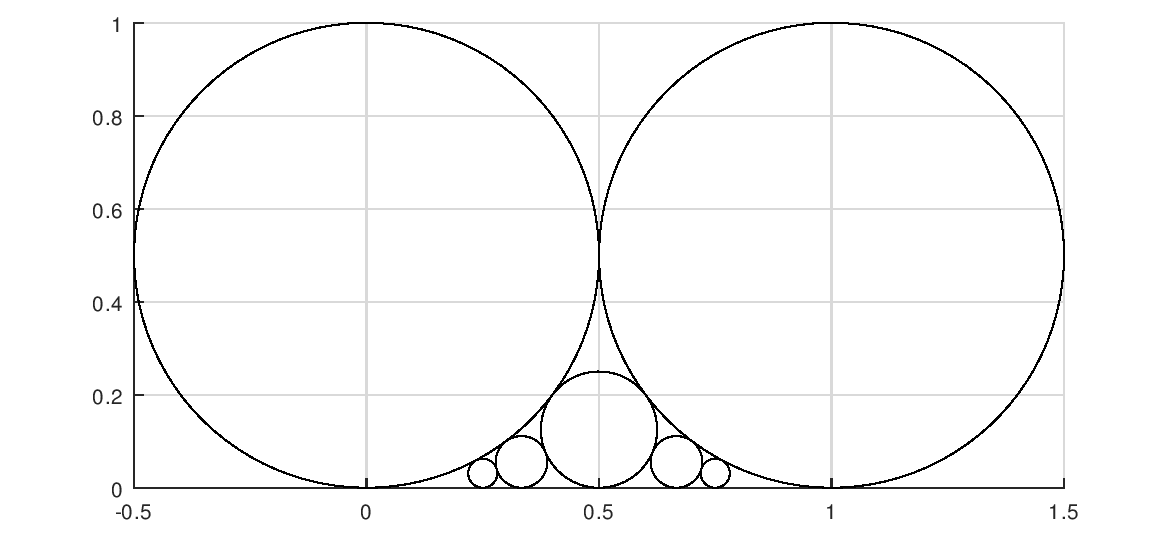
\includegraphics[scale=0.6]{fordovi_krogi.png}
\caption{Fordovi krogi na intervalu $[0,1]$ s polmeri $\protect{\frac{1}{2}}$, $\protect{\frac{1}{8}}$, $\protect{\frac{1}{18}}$ in $\protect{\frac{1}{32}}$.}
\end{center}
\end{figure}

Ker so Fordovi krogi definirani za vsak okrajšan ulomek, lahko poljubnemu racionalnemu številu enolično priredimo Fordov krog. Iz analize vemo, da je množica racionalnih števil gosta podmnožica množice realnih števil, abscisna os pa je geometrijska predstavitev le-te. Zato poljubno majhen interval na abscisni osi vsebuje neskončno mnogo dotikališč Fordovih krogov.

Zaradi simetrije je Fordove kroge dovolj obravnavati na intervalu $[0,1]$, obenem pa se zavedati, da jih lahko periodično razširimo na celotno realno os. V nadaljevanju bomo s pojmom množica Fordovih krogov označevali množico Fordovih krogov z dotikališči na intervalu $[0,1]$.

\begin{opomba}
Iz definicije zaradi pogoja o tujosti števil $p$ in $q$ neposredno sledi, da je množica Fordovih krogov v bijekciji s Fareyevim zaporedjem.
\end{opomba}

% konstrukcija pravokotnega trikotnika
Oglejmo si konstrukcijo pravokotnega trikotnika, določenega s parom Fordovih krogov, ki bo ključna pri dokazovanju trditev v tem poglavju. Izberimo okrajšana ulomka $\frac{a}{b}$ in $\frac{c}{d}$, ter jima priredimo ustrezna Fordova kroga. Naj bosta $A$ središče Fordovega kroga C($\frac{a}{b}$) in $B$ središče Fordovega kroga C($\frac{c}{d}$). Če je $b<d$, kar pomeni, da je polmer kroga C($\frac{a}{b}$) večji od polmera kroga C($\frac{c}{d}$), točko $C$ določimo kot presečišče navpične premice skozi točko $A$ z vodoravno premico skozi točko $B$. Sicer je $b>d$, točka $C$ pa presečišče navpične premice skozi točko $B$ z vodoravno premico skozi točko $A$. Primer, ko velja $b=d$, nam da izrojen trikotnik, zato ga izpustimo. Povežimo središči obeh krogov. Točki $D$ in $E$ naj bosta presečišči daljice $AB$ s Fordovima krogoma C($\frac{a}{b}$) in C($\frac{c}{d}$).

Vemo, da se kroga dotikata abscisne osi zaporedoma v točkah $\frac{a}{b}$ in $\frac{c}{d}$, njuna polmera pa merita $\frac{1}{2b^2}$ in $\frac{1}{2d^2}$. Od tod lahko izračunamo razdalje $|AB|$, $|AC|$ in $|BC|$.
Po konstrukciji je trikotnik $ABC$ pravokoten s pravim kotom v oglišču $C$, zato velja Pitagorov izrek
\begin{equation}
\label{Eq:Pitagora}
|AB|^2 = |AC|^2 + |BC|^2. 
\end{equation}

% slika pravokotni trikotnik
\begin{figure}[h!]
\begin{center}
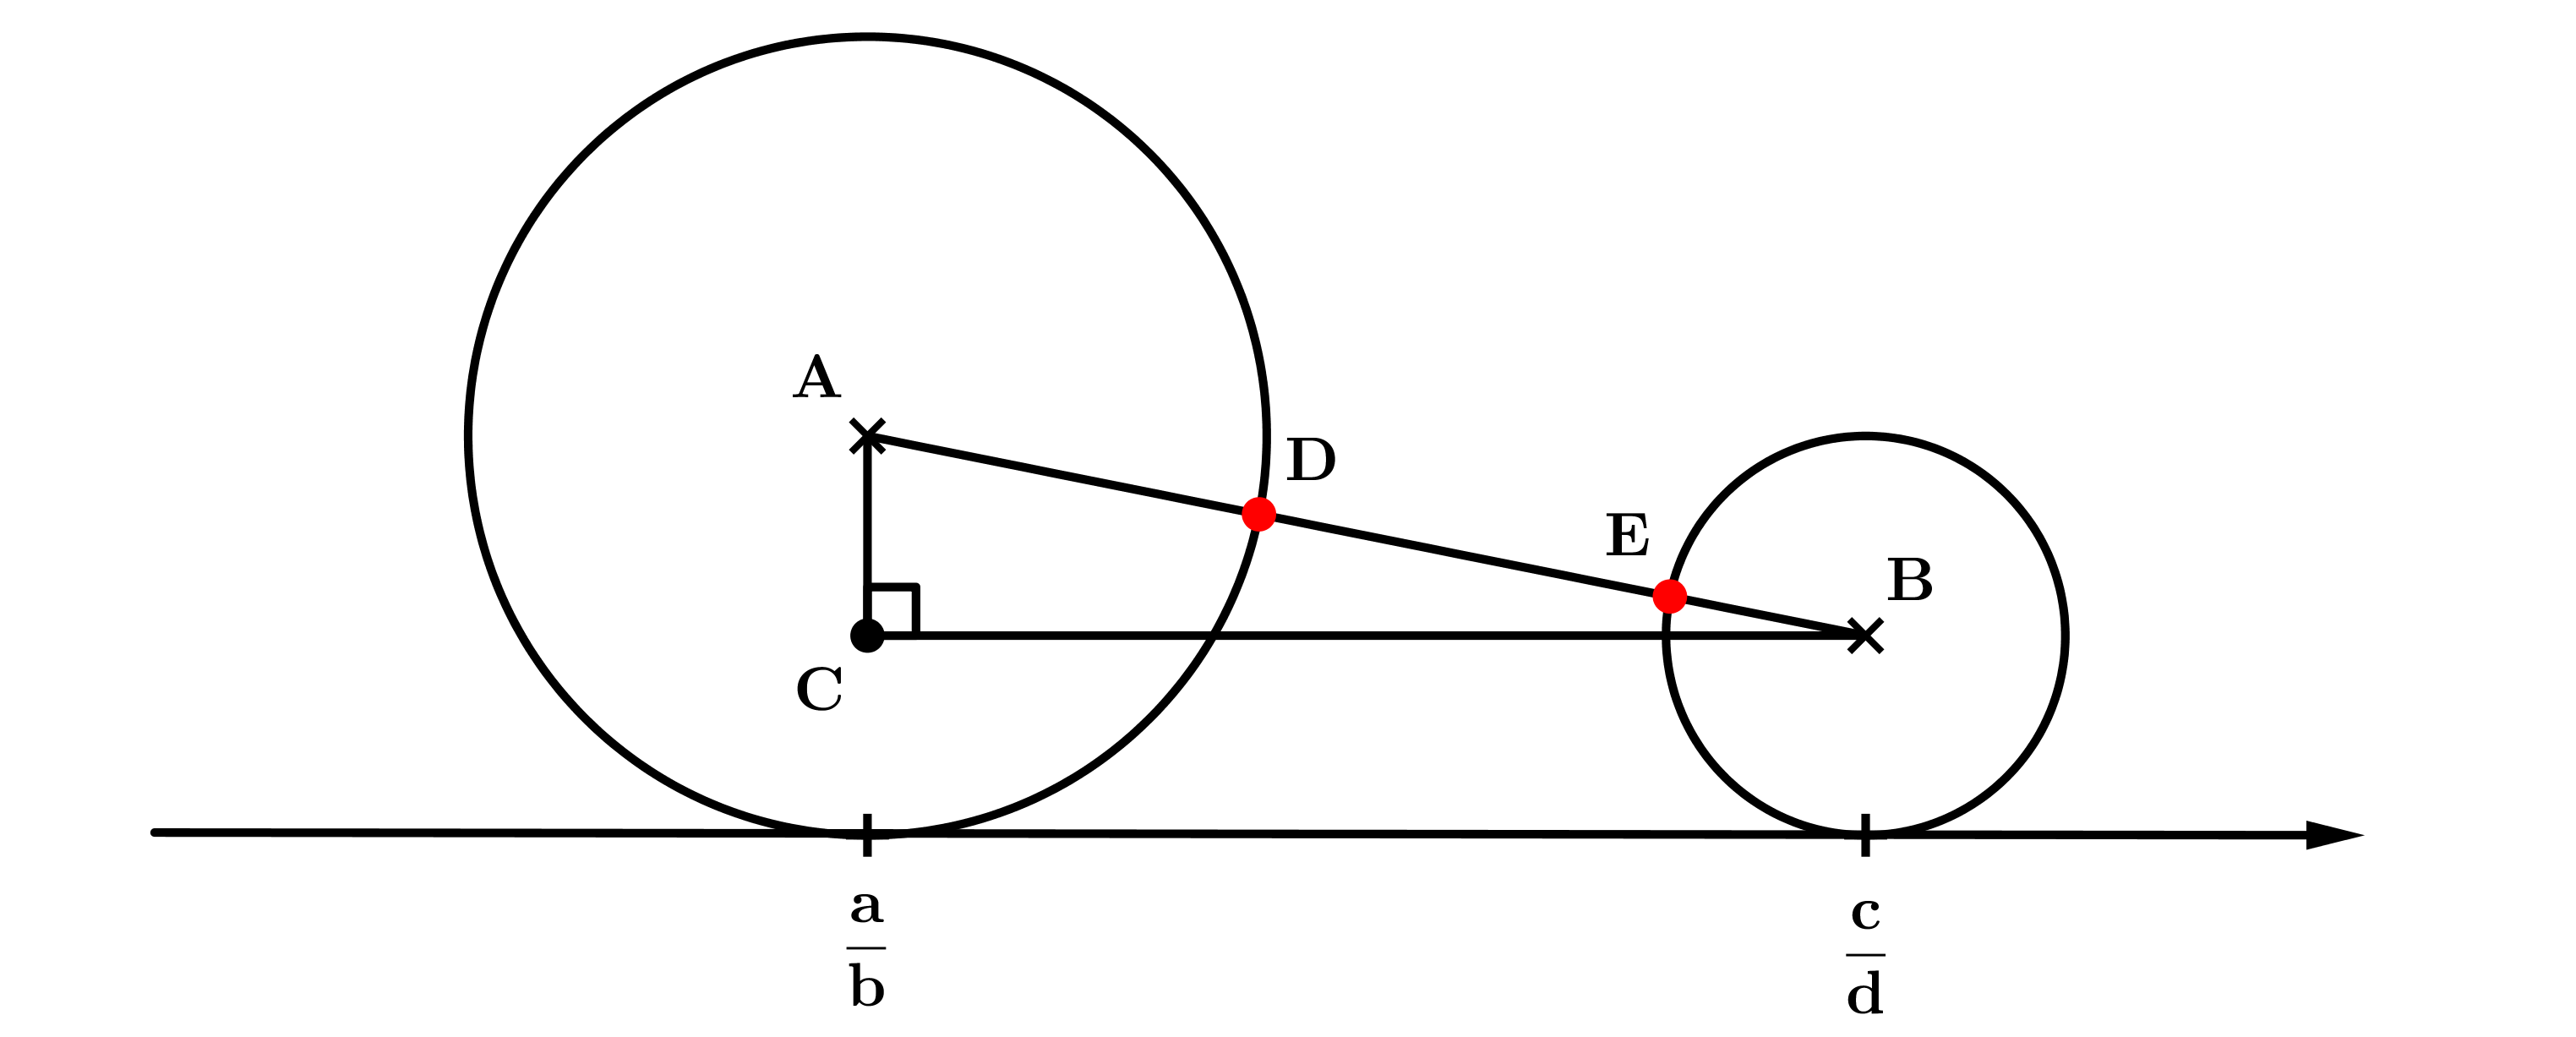
\includegraphics[scale=0.55]{pitagora1.png}
\caption{Konstrukcija pravokotnega trikotnika, ki pripada paru Fordovih krogov. Slika prikazuje primer, ko je $b<d$.}
\label{Fig:Pitagora}
\end{center}
\end{figure}

\begin{opomba}
Enačba~\ref{Eq:Pitagora} je neodvisna od relacije med polmeroma Fordovih krogov; velja tako v primeru, ko je $b>d$, kot za $b<d$.
\end{opomba}
%

\begin{trditev}
\label{trd:FordDisjTang}
Fordova kroga, ki pripadata različnima okrajšanima ulomkoma, sta bodisi tangentna bodisi disjunktna.
\end{trditev}

\begin{dokaz}
Konstruirajmo pravokotni trikotnik, kot je opisano zgoraj in zapišimo Pitagorov izrek iz enačbe~\eqref{Eq:Pitagora}.
Dolžine stranic trikotnika izrazimo z $a, b, c$ in $d$, kar nam da enakost
%
\begin{align}
|AB|^2 
  &= \left ( \left| \frac{1}{2b^2} - \frac{1}{2d^2} \right| \right)^2  + \left ( \left| \frac{c}{d} - \frac{a}{b} \right| \right )^2 \nonumber \\ 
  &= \frac{1}{4b^4} - \frac{1}{2b^2d^2} + \frac{1}{4d^4} + \left (\frac{bc-ad}{bd} \right )^2 \nonumber \\
  &= \left (\frac{1}{2b^2} + \frac{1}{2d^2} \right )^2 - \frac{1}{b^2d^2} + \frac{(bc-ad)^2}{b^2d^2} \nonumber \\
  &= (|AD| + |EB|)^2 + \frac{(bc-ad)^2-1}{b^2d^2}.
\end{align}

Če je $|bc-ad|>1$, je $|AB|^2 > (|AD| + |EB|)^2$, zato je $|AB| > |AD| + |EB|$ in Fordova kroga C($\frac{a}{b}$) in C($\frac{c}{d}$) sta disjunktna.

Če je $|bc-ad|=1$, je $|AB|^2 = (|AD| + |EB|)^2$, zato je $|AB| = |AD| + |EB|$ in Fordova kroga C($\frac{a}{b}$) in C($\frac{c}{d}$) sta tangentna.

Če je $|bc-ad|<1$, je $bc-ad = 0,$ saj smo v množici celih števil. Sledi $\frac{a}{b} = \frac{c}{d},$ kar vodi v protislovje s predpostavko trditve.
Torej sta Fordova kroga res bodisi tangentna bodisi disjunktna.
\end{dokaz}

%%%%%%%%%%%%%%%%%%%%%%%%%%%%%%%%%%%%%%%%%%%%%%%%%%%%%%%%%%%%%%%%%%%%%%%%%
% Fordovi sosedi
\subsection{Fordovi sosedi}

V poglavju o Fareyevem zaporedju smo dokazali lastnosti mediante in Fareyevih sosedov. Izkaže se, da imata ti dve lastnosti geometrijski pomen. Pokazali bomo namreč, da veljata tudi za tangentne Fordove kroge. V nadaljevanju bomo konstruirali vse tangentne Fordove kroge danega kroga in si ogledali še eno lastnost paroma tangentnih Fordovih krogov.

\begin{trditev}[Lastnost Fordovih sosedov]
\label{trd:FordTangentnost}
Fordova kroga C($\frac{a}{b}$) in C($\frac{c}{d}$) sta tangentna natanko tedaj, ko velja \( |bc-ad|=1. \)
\end{trditev}

\begin{dokaz}
%
Ponovno konstruirajmo pravokotni trikotnik kot v prejšnjem razdelku. Implikacijo v levo smo že izpeljali, zato si oglejmo še implikacijo v desno.

Denimo, da sta Fordova kroga C($\frac{a}{b}$) in C($\frac{c}{d}$) tangentna. Potem za pravokotni trikotnik, ki ga določata, velja Pitagorov izrek 
\[ |AC|^2 + |BC|^2 = |AB|^2 \] oziroma
\[ \left ( \left | \frac{1}{2b^2} - \frac{1}{2d^2} \right | \right )^2 + \left ( \left| \frac{c}{d} - \frac{a}{b} \right| \right )^2 = \left (\frac{1}{2b^2} + \frac{1}{2d^2} \right )^2. \]
Ko odpravimo oklepaje, opazimo, da se nekateri členi odštejejo. Nato odpravimo ulomke in novo enakost poenostavimo. Dobimo
\begin{align*}
\frac{1}{4b^4} - \frac{1}{2b^{2}d^{2}} + \frac{1}{4d^4} + \frac{c^2}{d^2} - \frac{2ac}{bd} + \frac{a^2}{b^2} &= \frac{1}{4b^4} + \frac{1}{2b^{2}d^{2}} + \frac{1}{4d^4}, \\
b^{2}c^{2} - 2abcd + a^{2}d^{2} &= 1, \\
(bc-ad)^2 &= 1, \\
|bc-ad|&=1.
\end{align*}
kar smo želeli pokazati.
\end{dokaz}

\begin{definicija}
Tangentna Fordova kroga imenujemo \emph{Fordova soseda}.
\end{definicija}

\begin{trditev}[Lastnost mediante za Fordove kroge]
Naj bosta C($\frac{a}{b}$) in C($\frac{c}{d}$) Fordova soseda. Tedaj obstaja enolično določen Fordov krog C($\frac{a+c}{b+d}$) in je tangenten na izbrana kroga. Imenujemo ga \emph{medianta Fordovih krogov}.
\end{trditev}

\begin{dokaz}
Po definiciji Fordovih krogov vemo, da sta $\frac{a}{b}$ in $\frac{c}{d}$ okrajšana ulomka in zaradi tangentnosti pripadajočih Fordovih krogov Fareyeva soseda v nekem Fareyevem zaporedju (razširjenem na celotno realno os). Po lemi~\ref{lema:MediantaOkrUlom} je njuna medianta $\frac{a+c}{b+d}$ tudi okrajšan ulomek, torej obstaja natanko en Fordov krog C($\frac{a+c}{b+d}$). 

Dokažimo še, da je Fordov krog C($\frac{a+c}{b+d}$) tangenten na izbrana kroga. Ker sta C($\frac{a}{b}$) in C($\frac{c}{d}$) Fordova soseda, velja zveza 
\( |bc-ad|=1. \)
Če jo nekoliko preoblikujemo, dobimo
\[ |bc-ad|=|bc-ad+cd-cd|=|(b+d)c-(a+c)d|=1, \]
od koder sledi, da sta Fordova kroga C($\frac{a+c}{b+d}$) in C($\frac{c}{d}$) tangentna.
Podobno
\[ |bc-ad|=|bc-ad+ab-ab|=|(a+c)b-(b+d)a|=1 \]
pomeni, da sta Fordova kroga C($\frac{a}{b}$) in C($\frac{a+c}{b+d}$) tangentna.
\end{dokaz}

% konstrukcija Fordovih sosedov
Naslednji izrek pove, kako konstruiramo množico vseh Fordovih sosedov danega Fordovega kroga. Izrek in dokaz sledita \cite[poglavje 2, Theorem 3, str.~588--589]{ford}.

\begin{izrek}
Naj bosta kroga C($\frac{p}{q}$) in C($\frac{P}{Q}$) Fordova soseda. Vse Fordove sosede Fordovega kroga C($\frac{p}{q}$) lahko zapišemo v obliki C($\frac{P_n}{Q_n}$), kjer je $\frac{P_n}{Q_n} = \frac{P+np}{Q+nq}$ in $n$ preteče vsa cela števila.
\end{izrek}

\begin{dokaz}
%
Najprej dokažimo, da sta Fordova kroga C($\frac{p}{q}$) in C($\frac{P_n}{Q_n}$) res Fordova soseda. Računajmo
\[ |qP_{n} - pQ_{n}| = |q(P+np) - p(Q+nq)| = |qP+qnp-pQ-pnq| = |qP-pQ| = 1. \]
Zadnja enakost velja po predpostavki, saj sta C($\frac{p}{q}$) in C($\frac{P}{Q}$) Fordova soseda.

Sedaj preverimo, če obstajajo še Fordovi sosedi, ki niso zgornje oblike. Opazovali bomo množico Fordovih krogov $\mathcal{M} = \{ \mathrm{C}(\frac{P_n}{Q_n}); n\in\Z \}.$
Iz računa
\begin{align}
|Q_{n}P_{n+1} - P_{n}Q_{n+1}| 
  &= |(Q+nq)(P+(n+1)p) - (P+np)(Q+(n+1)q)| \nonumber \\ 
  &= |QP + (n+1)Qp + nPq + n(n+1)pq \nonumber \\
  &   - PQ - (n+1)Pq - npQ - n(n+1)pq| \nonumber \\
  &= |Qp - Pq| \nonumber \\
  &= 1
\end{align}
sledi, da sta zaporedna elementa zaporedja $\mathcal{M}$ Fordova soseda. Ulomek $\frac{P_n}{Q_n}$, ki predstavlja Fordov krog C($\frac{P_n}{Q_n}$), lahko zapišemo kot
\begin{align}
\frac{P_n}{Q_n}
  &= \frac{P+np}{Q+nq} = \frac{Pq+npq}{q(Q+nq)} = \frac{Pq+npq+pQ-pQ}{q(Q+nq)} \nonumber \\
  &= \frac{p(Q+nq) + (Pq-pQ)}{q(Q+nq)} = \frac{p}{q} + \frac{Pq-pQ}{q(Q+nq)} \nonumber \\
  &= \frac{p}{q} \pm \frac{1}{q(Q+nq)} = \frac{p}{q} \pm \frac{1}{q^2 \left (n+\frac{Q}{q} \right)}.
\end{align}
%
\begin{figure}[h!]
\begin{center}
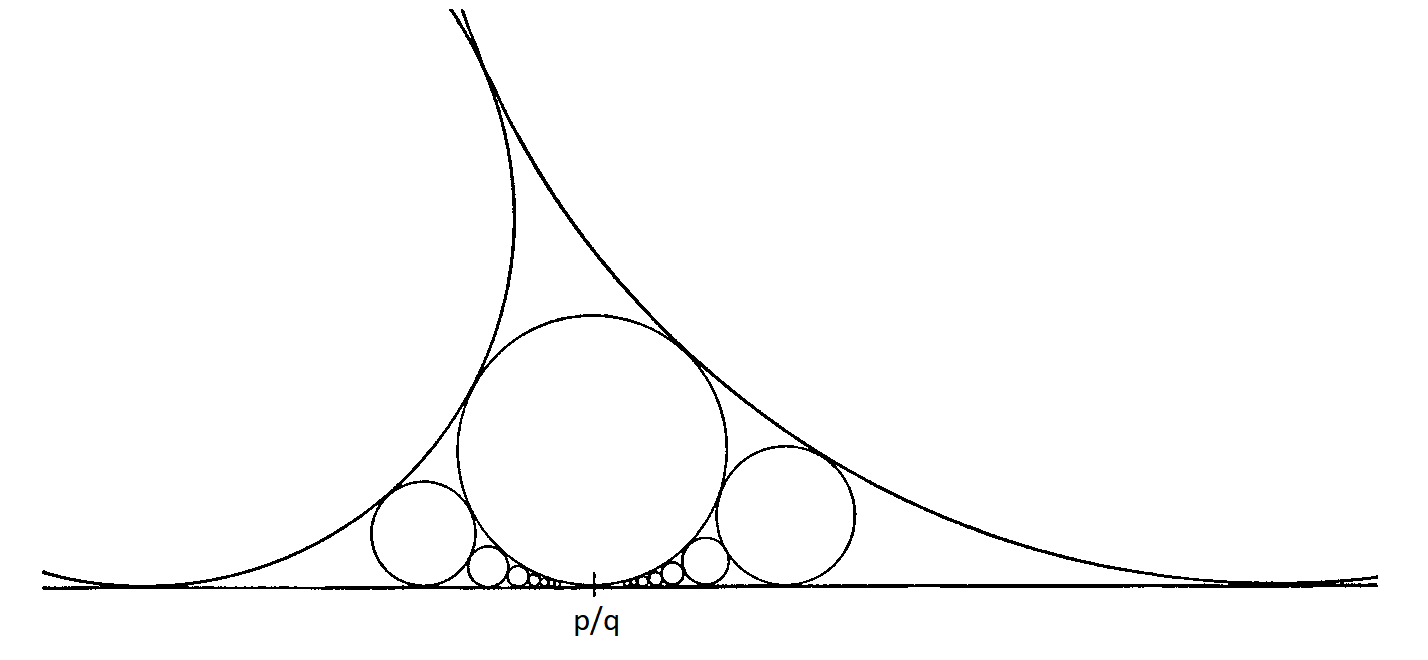
\includegraphics[scale=0.4]{ford_obroc.png}
\caption{Fordov krog C($\frac{p}{q}$) in nanj tangentni Fordovi krogi iz množice $\mathcal{M}$. Vir slike je~\cite[poglavje 2, Figure 2, str.~589]{ford}.}
\end{center}
\end{figure}
%
V limiti, ko gre $n$ preko vseh meja, gre $\frac{P_n}{Q_n}$ proti $\frac{p}{q}.$
Opazimo, da Fordovi krogi oblike C($\frac{P_n}{Q_n}$) geometrijsko tvorijo ``obroč'' okoli Fordovega kroga C($\frac{p}{q}$). Z njim so namreč vsi tangentni, prav tako pa so tangentni tudi na svojega predhodnika in naslednika v zaporedju $\mathcal{M}$. Njihova dotikališča z abscisno osjo konvergirajo proti točki $\frac{p}{q},$ ki je dotikališče danega Fordovega kroga C($\frac{p}{q}$), zaradi medsebojne tangentnosti pa so njihovi polmeri vse manjši. Zato ne obstaja Fordov krog, tangenten na C($\frac{p}{q}$), ki ni zgornje oblike in ne seka katerega izmed krogov iz zaporedja $\mathcal{M}$.
%
\end{dokaz}

% Pitagorejske trojice
%
V prejšnjem razdelku smo konstruirali pravokotni trikotnik, določen s središčema tangentnih Fordovih krogov in presečiščem premic skozi središči. Spomnimo se znane definicije iz teorije števil, ki izhaja iz evklidske geometrije. 

\begin{definicija}
Trojica naravnih števil $(a,b,c)$, za katero velja $a^2+b^2=c^2$, se imenuje \emph{pitagorejska trojica}\footnote{Pojem pitagorejska trojica nosi ime starogrškega matematika Pitagore (okoli 570~pr.~n.~št.--495~pr.~n.~št.), ki ga poznamo predvsem po Pitagorovem izreku.}.
Pitagorejska trojica je \emph{primitivna}, če števila $a$, $b$, in $c$ nimajo skupnega faktorja.
\end{definicija}

\begin{trditev}
Pravokotna trikotnika, ki pripadata poljubnima paroma Fordovih sosedov, določata različni primitivni pitagorejski trojici.
\end{trditev}

\begin{dokaz}
%
Naj bosta C($\frac{a}{b}$) in C($\frac{c}{d}$) ter C($\frac{a'}{b'}$) in C($\frac{c'}{d'}$) poljubna različna para Fordovih sosedov. Brez škode za splošnost naj velja $b<d$ in $b'<d'$. Naj prvemu paru Fordovih sosedov pripada pravokotni trikotnik $ABC$, drugemu paru pa pravokotni trikotnik $A'B'C'$. Trdimo, da si trikotnika nista podobna.

Pa denimo, da sta si trikotnika $ABC$ in $A'B'C'$ podobna. Tedaj obstaja tako naravno število $\lambda\ne{1}$, da za dolžine stranic obeh pravokotnih trikotnikov veljajo naslednje zveze:
%
\begin{equation}
\label{Eq:Pit1}
\frac{1}{2b^2}-\frac{1}{2d^2} = \lambda \left (\frac{1}{2b'^2}-\frac{1}{2d'^2} \right ),
\end{equation}
%
\begin{equation}
\label{Eq:Pit2}
\frac{1}{2b^2}+\frac{1}{2d^2} = \lambda \left (\frac{1}{2b'^2}+\frac{1}{2d'^2} \right ),
\end{equation}
%
\begin{equation}
\label{Eq:Pit3}
\frac{c}{d}-\frac{a}{b} = \lambda \left (\frac{c'}{d'}-\frac{a'}{b'} \right ).
\end{equation}
%
Če seštejemo enačbi~\eqref{Eq:Pit1} in \eqref{Eq:Pit2}, dobimo
%
\begin{align}
\label{Eq:Pit4}
\frac{1}{b^2} &= \lambda \frac{1}{b'^2}, \nonumber \\
b'^2 &= \lambda b^2, \nonumber \\
b' &= \sqrt\lambda b.
\end{align}
%
Enačbo~\eqref{Eq:Pit3} lahko poenostavimo, saj gre za para Fordovih sosedov. Velja
\begin{equation}
\label{Eq:Pit5}
\pm \frac{1}{bd} = \frac{bc-ad}{bd} = \frac{c}{d}-\frac{a}{b} = \lambda \left (\frac{c'}{d'}-\frac{a'}{b'} \right ) = \lambda \frac{b'c'-a'd'}{b'd'} = \pm \lambda \frac{1}{b'd'}.
\end{equation}
%
Oba predznaka sta enaka. Iz enakosti~\eqref{Eq:Pit4} in~\eqref{Eq:Pit5} sledi 
%
\begin{align}
\label{Eq:Pit6}
\frac{1}{bd} &=\lambda \frac{1}{\sqrt\lambda bd'}, \nonumber \\
\frac{1}{d} &= \frac{\sqrt\lambda}{d'}, \nonumber \\
d' &= \sqrt\lambda d.
\end{align}
%
Nazadnje še v pogoj za tangentnost krogov C($\frac{a'}{b'}$) in C($\frac{c'}{d'}$) vstavimo zvezi~\eqref{Eq:Pit4} in~\eqref{Eq:Pit6}, kar nam da
%
\begin{align}
|b'c'-a'd'| &= 1, \nonumber \\
|\sqrt\lambda bc' - a' \sqrt\lambda d| &= 1, \nonumber \\
\sqrt\lambda |bc'-a'd| &= 1.
\end{align}
%
To pa je možno le tedaj, ko je $\lambda=1.$ Prispeli smo do protislovja, kar pomeni, da si trikotnika nista podobna.
%
Zakaj so pitagorejske trojice primitivne?
Če so dolžine stranic posameznega pravokotnega trikotnika paroma tuja naravna števila, že določajo primitivno pitagorejsko trojico.
Če imajo ta naravna števila skupni celoštevilski faktor, jih z njim delimo (to geometrijsko pomeni, da konstruiramo podobni trikotnik), kar nam da primitivno pitagorejsko trojico.
Če pa so dolžine stranic racionalna števila, jih pomnožimo z najmanjšim skupnim večkratnikom njihovih imenovalcev in dobimo enega izmed zgornjih primerov.
\end{dokaz}

\begin{opomba}
Enoličnost pitagorejskih trojic je določena do simetrij Fordovih krogov natančno. Fordovi krogi so namreč tako kot Fareyevo zaporedje simetrični okoli vrednosti $\frac{1}{2}$.
\end{opomba}

%%%%%%%%%%%%%%%%%%%%%%%%%%%%%%%%%%%%%%%%%%%%%%%%%%%%%%%%%%%%%%%%%%%%%%%%%
% Posplositve
\subsection{Posplošeni Fordovi krogi}

Do sedaj smo se ukvarjali s Fordovimi krogi, ki so enolično določeni z racionalnim številom. Natančneje, danemu okrajšanemu ulomku $\frac{p}{q}$ smo priredili Fordov krog na zgornji polravnini evklidske ravnine, ki se abscisne osi dotika v točki $\frac{p}{q}$, njegov polmer pa meri $\frac{1}{2q^2}.$
Nadaljujemo lahko s splošnejšimi Fordovimi krogi, ki so definirani na povsem enak način, le da imajo polmer enak $\frac{1}{2hq^2},$ pri čemer je $h$ poljubno realno število. Imenujemo jih tudi Speiserjevi\footnote{Andreas Speiser, 10.\ 6.\ 1885--12.\ 10.\ 1970, švicarski matematik, ki se je ukvarjal s teorijo števil in teorijo grup.} krogi. Če izberemo $h=1,$ dobimo običajne Fordove kroge.
Posplošeni Fordovi krogi so povezani z geometrijo modularnih grup in teorijo kvadratnih form.

% slika posplosenih Fordovih krogov
\begin{figure}[h!]
\begin{center}
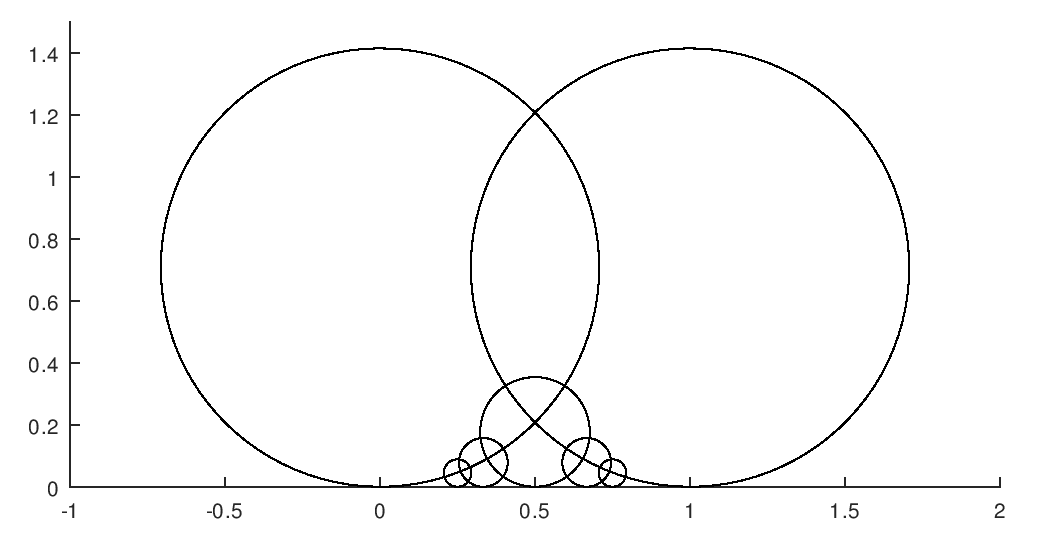
\includegraphics[scale=0.6]{posploseni_fordovi_krogi.png}
\caption{Posplošeni Fordovi krogi, kjer je $\protect{h=\sqrt{2}/2}$. Sosednji posplošeni Fordovi krogi niso tangentni, pač pa se sekajo.}
\label{Fig:PosplFord}
\end{center}
\end{figure}

%%%%%%%%%%%%%%%%%%%%%%%%%%%%%%%%%%%%%%%%%%%%%%%%%%%%%%%%%%%%%%%%%%%%%%%%%
% Fordove krogle
\subsection{Fordove krogle}

V tem razdelku bomo sledili \cite[poglavje 8]{ford}.
Tokrat naj bosta števili $p$ in $q$ elementa množice Gaussovih celih števil, ki je definirana kot $\mathbb{Z}\left[{i}\right] = \{a+bi; a,b \in \Z \}.$ Zapišimo $p = p'+ip''$ in $q = q'+iq'',$ kjer so $p', p'', q', q'' \in \Z.$ Definirajmo ulomek
\begin{align} 
\frac{p}{q} = \frac{p'+ip''}{q'+iq''} = \frac{(p'+ip'')(q'-iq'')}{(q'+iq'')(q'-iq'')} = \frac{p'q'+p''q''}{q'^2+q''^2} + i \frac{p''q'-p'q''}{q'^2+q''^2},
\end{align}
ki pripada kompleksnim številom, ter okrajšajmo posebej njegov realni in imaginarni del. Geometrijsko predstavlja točko v Gaussovi $xy$-ravnini z realno in imaginarno komponento. Gaussovo ravnino postavimo v prostor, določen z osjo $z$, pravokotno na Gaussovo ravnino, in opazujmo podprostor, ki pripada pozitivnim vrednostim na $z$-osi. Analogno Fordovim krogom v ravnini pridemo do naslednjega pojma. 

\begin{definicija}
\emph{Fordova krogla} S($\frac{p}{q}$), kjer je $\frac{p}{q}$ okrajšan ulomek v množici kompleksnih števil, je krogla v zgornjem polprostoru, definiranem kot zgoraj, ki se $xy$-ravnine dotika v točki, določeni s $\frac{p}{q}$, njen polmer pa meri $\frac{1}{2|q|^2}.$
\end{definicija}

\begin{figure}[h!]
\begin{center}
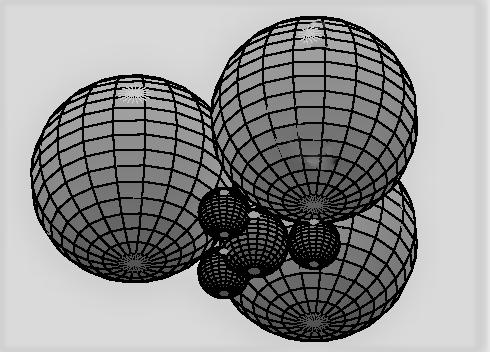
\includegraphics[scale=1]{fordove_krogle1.png}
\caption{Fordove krogle.}
\end{center}
\end{figure}

% lastnosti
Na analogen način trditvam, ki opisujejo lastnosti Fordovih krogov, lahko izpeljemo in dokažemo lastnosti Fordovih krogel. Omenimo le nekatere izmed njih.

Poljubno majhen zaprt pravokotnik v $xy$-ravnini vsebuje neskončno mnogo dotikališč Fordovih krogel.

Spomnimo se konstrukcije pravokotnega trikotnika, določenega z dvema Fordovima krogoma. Naj točki $\frac{p}{q}$ in $\frac{P}{Q}$ določata Fordovi krogli ter konstruirajmo pravokotni trikotnik $ABC$ kot prej. Iz zveze
\begin{align*}
|AB|^2 
  &= \left |\frac{P}{Q} - \frac{p}{q} \right|^2 + \left |\frac{1}{2|Q|^2} - \frac{1}{2|q|^2} \right|^2 = \frac{|Pq-pQ|^2-1}{|Q|^2|q|^2} + (|AD| + |EB|)^2
\end{align*}
sledi:
če je $|Pq-pQ|>1,$ je $|AB|>|AD|+|EB|$ in krogli sta disjunktni;
sicer je $|Pq-pQ|=1,$ zato je $|AB|=|AD|+|EB|$ in krogli sta tangentni.

Naj bosta S($\frac{p}{q}$) in S($\frac{P}{Q}$) tangentni Fordovi krogli. Kot prej vse tangentne Fordove krogle na dano kroglo S($\frac{p}{q}$) pripadajo vrednostim
\begin{equation}
\frac{P_n}{Q_n} = \frac{P+np}{Q+nq},
\end{equation}
le da tokrat $n$ pripada množici Gaussovih celih števil. 
Nadalje nas zanima, koliko Fordovih krogel je tangentnih na kroglo S($\frac{P_n}{Q_n}$).
Uporabimo pogoj za tangentnost, ki smo ga izpeljali. Računajmo
\begin{align} 
|P_{n}Q_{m} - P_{m}Q_{n}| 
  &= |(P+np)(Q+mq) - (P+mp)(Q+nq)| \nonumber \\
  &= |PQ+mPq+npQ+mnpq-PQ-nPq-mpQ-mnpq| \nonumber \\
  &= |Pq-pQ| |m-n| = 1.
\end{align}
%
Sledi, da je $|m-n|=1,$ torej je razlika $m-n \in \{1, -1, i, -i \}.$ Ugotovili smo, da je vsaka Fordova krogla, ki je tangentna na dano Fordovo kroglo, tangentna še na štiri druge Fordove krogle, ki so tangentne na obe.

%%%%%%%%%%%%%%%%%%%%%%%%%%%%%%%%%%%%%%%%%%%%%%%%%%%%%%%%%%%%%%%%%%%%%%%%%% 
% Mobiusove transformacije na Fordovih krogih
\subsection{M\"{o}biusove transformacije na Fordovih krogih}

Zaenkrat smo Fordove kroge obravnavali s pomočjo geometrijskih sredstev. V tem razdelku si bomo z algebro pomagali do nekaterih že znanih rezultatov o Fordovih krogih.
Geometrijske objekte si bomo predstavljali v kompleksni ravnini, torej bo točka s koordinatama $(x,y)$ opisana s kompleksnim številom $z=x+iy$, pri čemer sta $x, y, \in \mathbb{R}$.

% Mobiusova transformacija
Najprej se spomnimo naslednjega pojma iz kompleksne analize.
\begin{definicija}
\label{def:MobTransformacija}
Preslikava \( f \colon \mathbb{CP}^{1} \rightarrow \mathbb{CP}^{1} \), definirana s predpisom \( f(z) = \frac{az+c}{bz+d} \), kjer so $a,b,c,d \in \mathbb{C}$ in $ad-bc \neq 0$, se imenuje \emph{M\"{o}biusova transformacija}.
\end{definicija} 

\begin{opomba}
Simbol $ \mathbb{CP}^{1}$ označuje \emph{Riemannovo sfero}, to je kompaktifikacijo kompleksne ravnine z eno točko, kar zapišemo kot $\mathbb{CP}^{1} = \mathbb{C} \cup \{\infty\}$.
\end{opomba}

\begin{opomba}
Števila $a,b,c,d$ lahko pomnožimo s poljubnim neničelnim kompleksnim številom, zato brez škode za splošnost predpostavimo, da je $ad-bc=1$.

V našem primeru bo dovolj obravnavati le $a,b,c,d \in \mathbb{Z}$.
\end{opomba}

M\"{o}biusova transformacija je meromorfna in bijektivna preslikava z inverzom, ki je spet take oblike, identična preslikava $id(z)=z$ je M\"{o}biusova transformacija, prav tako je kompozitum M\"{o}biusovih transformacij M\"{o}biusova transformacija. Množica takih preslikav torej tvori grupo za kompozitum. 
Preslikavo $f$ lahko zapišemo v matrični obliki
\[
\mathbf{A}\ =
\left[
\begin{array}{cc}
a & c \\
b & d \\
\end{array}
\right],
\]
kjer so $a,b,c,d \in \mathbb{Z}$. Ker velja $ad-bc=1$, je matrika $A \in {SL}_{2}(\mathbb{Z})$. Zato bomo M\"{o}biusove transformacije predstavljali kot elemente splošne linearne grupe ${SL}_{2}(\mathbb{Z})$.

% Delovanje grupe na množico
Pri izpeljavi rezultatov o Fordovih krogih je ključen pojem, ki ga v algebri pogosto uporabljamo.

\begin{definicija}
\emph{Delovanje grupe} $G$ na množico $M$ je taka preslikava \( \circ \colon G \times M \rightarrow M \), za katero velja:
\begin{enumerate}
	\item \( e \circ \alpha = \alpha \) za vsak $ \alpha \in M$, kjer je $e$ enota grupe $G$, 
	\item \( g \circ (h \circ \alpha) = (gh) \circ \alpha \) za vsak $\alpha \in M$ in vsaka $g,h \in G$.
\end{enumerate}

Ekvivalentno, delovanje grupe $G$ na množico $M$ je homomorfizem iz grupe $G$ v grupo permutacij množice $M$.
\end{definicija}

\begin{primer}
Naj bo $G$ grupa permutacij $n$ elementov, torej $G = S_{n}$, za množico $M$ pa izberimo $M = \{1,2, \ldots, n \}$.
Delovanje grupe $G$ na množico $M$ je preslikava \( \circ \colon G \times M \rightarrow M \) s predpisom \( (\pi, \alpha) \mapsto \pi(\alpha) = \pi \circ \alpha \).
\end{primer}

% Fordovi krogi
\begin{definicija}
Fordov krog C($\frac{1}{0}$), katerega polmer je neskončen, je premica $\mathbb{R} + i$.
\end{definicija}

\begin{figure}[h!]
\begin{center}
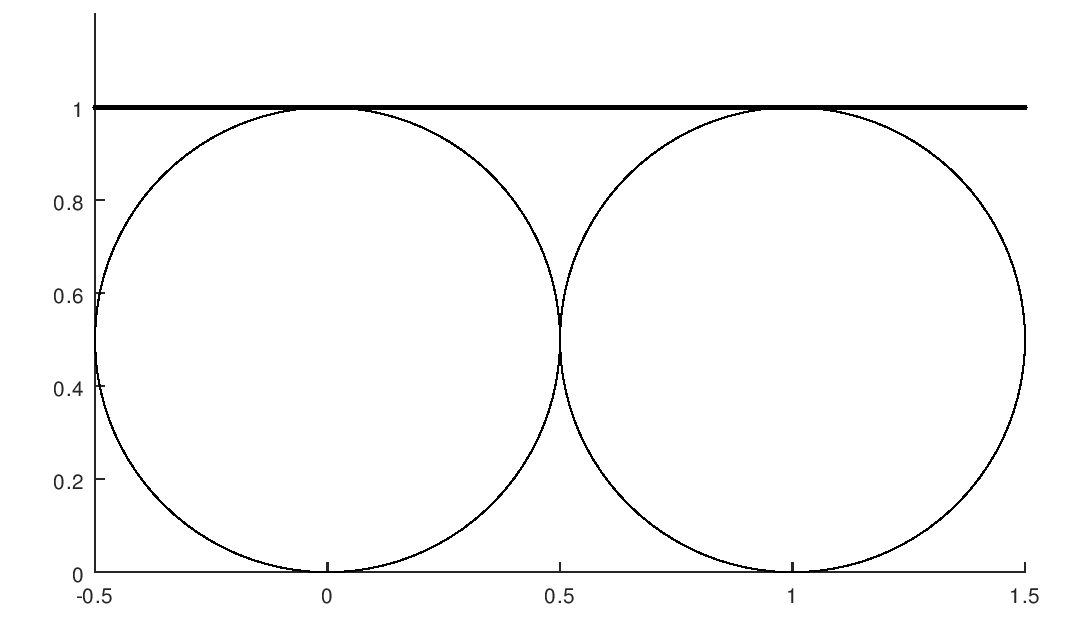
\includegraphics[scale=0.58]{fordovi_v_kompleksnem.png}
\caption{Fordovi krogi C($\frac{1}{0}$), C($\frac{0}{1}$) in C($\frac{1}{1}$) v kompleksni ravnini se dotikajo v točkah $i$, $1+i$ in $\frac{1}{2}+\frac{1}{2} i$.}
\end{center}
\end{figure}

V nadaljevanju tega razdelka bomo s pojmom množica Fordovih krogov označevali Fordove kroge na celotni realni osi vključno s krogom C($\frac{1}{0}$).

\begin{izrek}
\label{izr:MobDelovanje}
M\"{o}biusova transformacija $A \in {SL}_{2}(\mathbb{Z})$ slika Fordove kroge v Fordove kroge.
\end{izrek}

\begin{dokaz}
Naj bo M\"{o}biusova transformacija dana z matriko 
\[
\mathbf{A}\ =
\left[
\begin{array}{cc}
a & c \\
b & d \\
\end{array}
\right]
\in {SL}_{2}(\mathbb{Z}).
\]
Vemo, da tovrstna preslikava slika premice in krožnice v premice in krožnice. Ideja dokaza je pokazati, da grupa ${SL}_{2}(\mathbb{Z})$ deluje na množico Fordovih krogov.

S krajšim računom se lahko prepričamo, da je grupa ${SL}_{2}(\mathbb{Z})$ generirana z matrikama 
\(
\left[
\begin{array}{cc}
1 & 1 \\
0 & 1 \\
\end{array}
\right]
\)
in
\(
\left[
\begin{array}{cc}
0 & -1 \\
1 & 0 \\
\end{array}
\right]
\).
To pomeni, da je vsako M\"{o}biusovo transformacijo moč zapisati kot kompozitum preslikav $z \mapsto z+1$ in $z \mapsto -\frac{1}{z}$, ki ustrezata zgornjima generatorjema. Trdimo, da M\"{o}biusova transformacija preslika Fordov krog v Fordov krog. 

Preslikava $z \mapsto z+1$ je translacija, zato zgornje očitno velja.

Kaj pa preslikava $z \mapsto -\frac{1}{z}$? Najprej si oglejmo splošen primer. Naj bo original Fordov krog s polmerom $r$ in središčem v $\alpha$, predstavljen z enačbo $ |z-\alpha|=r$. Prepišimo enačbo v
\begin{align}
(z-\alpha)( \bar{z}-\bar{\alpha}) &= r^2, \nonumber \\
z\bar{z} - \alpha \bar{z} - \bar{\alpha} z + \alpha \bar{\alpha} - r^2 &= 0
\end{align}
in označimo $R = \alpha \bar{\alpha} - r^2$. Polmer lahko izrazimo kot $r = \sqrt{|\alpha|^2-R}$.
%
Preslikajmo original s preslikavo $z \mapsto -\frac{1}{z}$. Enačba slike se glasi
\begin{align}
\label{Eq:MobSlika}
\left(-\frac{1}{z}\right)\left(-\frac{1}{\bar{z}}\right) + \alpha \frac{1}{\bar{z}} + \bar{\alpha} \frac{1}{z} + R &= 0, \nonumber \\
1 + \alpha z + \bar{\alpha} \bar{z} + Rz \bar{z} &= 0, \nonumber \\
z \bar{z} + \frac{\bar{\alpha}}{R} \bar{z} + \frac{\alpha}{R} z + \frac{1}{R} &= 0.
\end{align}
%
% p,q \neq 0

Sedaj vzemimo Fordov krog C($\frac{p}{q}$), za katerega velja $p,q \neq 0$. Njegov polmer meri $\frac{1}{2q^2}$, središče pa je v točki $\frac{p}{q} +i \frac{1}{2q^2}$.
Izračunajmo
\[ R = \alpha \bar{\alpha} - r^2 = \left(\frac{p}{q} + i\frac{1}{2q^2} \right) \left(\frac{p}{q} - i\frac{1}{2q^2} \right) - \frac{1}{4q^4} 
= \frac{p^2}{q^2} + \frac{1}{4q^4} - \frac{1}{4q^4} = \frac{p^2}{q^2} \]
in preverimo, da je slika izbranega Fordovega kroga prav tako Fordov krog. Res, središče slike je po enačbi~\eqref{Eq:MobSlika} v točki
\begin{align}
-\frac{\bar{\alpha}}{R} = - \frac{\frac{p}{q} - i \frac{1}{2q^2}}{\frac{p^2}{q^2}} = - \frac{q}{p} + i \frac{1}{2p^2},
\end{align}
polmer pa meri
\begin{align}
\sqrt{ \left| - \frac{\bar{\alpha}}{R} \right|^2 - \frac{1}{R} } = \sqrt{ \frac{\bar{\alpha}}{R} \frac{\alpha}{R} - \frac{1}{R} } 
= \frac{1}{R} \sqrt{|\alpha|^2 - R} =  \frac{1}{R} \frac{1}{2q^2} = \frac{q^2}{2p^2 q^2} = \frac{1}{2p^2}.
\end{align}
%
% p=0 ali q=0

Sliki Fordovih krogov C($\frac{0}{1}$) in C($\frac{1}{0}$) bomo obravnavali posebej. Preslikava $z \mapsto -\frac{1}{z}$ je M\"obiusova transformacija, ki slika premice in krožnice v premice in krožnice, krožnica pa je natanko določena s tremi točkami. Zato v našem primeru zadostuje poznati slike treh točk na Fordovem krogu. Izberimo točke $0$, $i$ in $\frac{1}{2} + \frac{1}{2} i$, ki ležijo na Fordovem krogu C($\frac{0}{1}$). Preslikajo se v točke $-\infty$, $i$ in $-1+i$; te ležijo na premici $\{x+i; x \in \mathbb{R} \}$, to je Fordovem krogu C($\frac{1}{0}$). Zato je slika kroga C($\frac{0}{1}$) Fordov krog C($\frac{1}{0}$). Ker je preslikava bijekcija, se Fordov krog C($\frac{1}{0}$) preslika v C($\frac{0}{1}$).

%
Dokazali smo, da preslikavi, ki generirata grupo M\"{o}biusovih transformacij, Fordov krog preslikata v Fordov krog. Ker identiteta slika Fordov krog vase in je kompozitum M\"{o}biusovih transformacij dobro definiran, grupa ${SL}_{2}(\mathbb{Z})$ res deluje na množico Fordovih krogov.
\end{dokaz}

% lastnost mediante in Mobiusova transformacija
\begin{lema}
Dana naj bosta Fordova kroga C($\frac{e}{f}$) in C($\frac{g}{h}$). M\"{o}biusova transformacija, ki deluje na množico Fordovih krogov, ohranja $|eh-fg|$.
\end{lema}

\begin{dokaz}
Kot v definiciji~\ref{def:MobTransformacija} zapišimo M\"{o}biusovo transformacijo v obliki $m(z) = \frac{az+c}{bz+d}$, kjer so $a,b,c,d \in \mathbb{Z}$ in velja $ad-bc=1$. 
Vzemimo Fordova kroga C($\frac{e}{f}$) in C($\frac{g}{h}$), ter poglejmo, kam se preslikata. 
Ker velja izrek~\ref{izr:MobDelovanje} in je Fordov krog enolično določen s točko, v kateri se dotika realne osi v kompleksni ravnini, je dovolj poznati sliko te točke.
Izračunajmo
\[ m \left(\frac{e}{f} \right) = \frac{a \frac{e}{f} + c}{b \frac{e}{f} + d} = \frac{ae + cf}{be + df}, \]
od koder sledi, da se Fordov krog C($\frac{e}{f}$) preslika v Fordov krog C($\frac{ae+cf}{be+df}$).
Podobno,
\[ m \left(\frac{g}{h} \right) = \frac{a \frac{g}{h} + c}{b \frac{g}{h} + d} = \frac{ag + ch}{bg + dh}, \]
zato se C($\frac{g}{h}$) preslika v C($\frac{ag+ch}{bg+dh}$).
Označimo \( e' = ae+cf, f' = be+df, g' = ag+ch \) in $h' = bg+dh$. Računajmo
\[ e'h'-f'g' = (ae+cf)(bg+dh) - (be+df)(ag+ch) = (ad - bc)(eh - fg), \]
katerega absolutna vrednost je enaka
\[ |e'h'-f'g'| = |ad-bc| |eh-fg| = |eh-fg|, \]
s čimer smo dokazali želeno enakost.
\end{dokaz}

Iz zgornjega neposredno sledi naslednja ugotovitev.

\begin{posledica}
\label{Posl:MobOhr1}
Dana naj bosta Fordova kroga C($\frac{e}{f}$) in C($\frac{g}{h}$). M\"{o}biusova transformacija, ki deluje na množico Fordovih krogov, ohranja $|eh-fg|=1$.
\end{posledica}

Sedaj bomo s pomočjo orodij, ki smo jih obravnavali v tem razdelku, ponovno dokazali že znano \emph{lastnost mediante za Fordove kroge}.

\begin{dokaz}[Dokaz lastnosti mediante za Fordove kroge z M\"{o}biusovimi transformacijami]
Kroga C($\frac{r}{s}$) in C($\frac{p}{q}$) naj bosta Fordova soseda. Naj bo Fordov krog C($\frac{k}{l}$) tangenten na oba. Trdimo, da je C($\frac{k}{l}$) medianta Fordovih krogov C($\frac{r}{s}$) in C($\frac{p}{q}$), torej je enak C($\frac{r+p}{s+q}$).

Vzemimo točke v dotikališčih Fordovih krogov C($\frac{r}{s}$), C($\frac{p}{q}$) in C($\frac{k}{l}$). Vemo, da za točke $\alpha$, $\beta$, $\gamma$ obstaja M\"{o}biusova transformacija, ki jih preslika v poljubne točke $\lambda$, $\mu$, $\nu$. Torej obstaja M\"{o}biusova transformacija $M$, ki izbrane točke v dotikališčih preslika v točke $i$, $\frac{1}{2}+\frac{1}{2}i$, $1+i$. Ker M\"{o}biusova transformacija slika Fordove kroge v Fordove kroge, mi pa poznamo sliki dveh točk na vsakem izmed krogov C($\frac{r}{s}$), C($\frac{p}{q}$) in C($\frac{k}{l}$), poznamo slike vseh treh Fordovih krogov. Te pa so točno C($\frac{1}{0}$), C($\frac{0}{1}$) in C($\frac{1}{1}$).

Sedaj bomo konstruirali zaporedje M\"{o}biusovih transformacij (kompozitum katerih je prav tako M\"{o}biusova transformacija). Začnimo s Fordovima sosedoma C($\frac{r}{s}$) in C($\frac{p}{q}$). Preslikava $M_{1}$ ju preslika v Fordova kroga C($\frac{1}{0}$) in C($\frac{0}{1}$) z medianto C($\frac{1}{1}$). Kot v prvem delu dokaza izberimo tri točke v dotikališčih in jih preslikajmo. Obstaja M\"{o}biusova transformacija $M_{2}$, ki Fordove kroge C($\frac{1}{0}$), C($\frac{0}{1}$) in C($\frac{1}{1}$) zaporedoma preslika v Fordove kroge C($\frac{a}{b}$) in C($\frac{c}{d}$) in C($\frac{a+c}{b+d}$). Nadaljujemo s transformacijo $M_{3}$, ki slednje preslika po vrsti v Fordove kroge C($\frac{1}{0}$), C($\frac{0}{1}$) in C($\frac{1}{1}$), in končajmo s transformacijo $M_{4}$, ki le-te preslika v Fordove kroge C($\frac{r}{s}$), C($\frac{p}{q}$) in C($\frac{r+p}{s+q}$).

Vse zgornje preslikave so M\"{o}biusove transformacije, ki ohranjajo medianto Fordovih krogov (saj velja posledica~\ref{Posl:MobOhr1} ter je C($\frac{1}{1}$) medianta C($\frac{1}{0}$) in C($\frac{0}{1}$)), zato tudi kompozitum $M_{4} \circ M_{3} \circ M_{2} \circ M_{1}$ ohranja medianto. Sledi, da je naš kandidat C($\frac{k}{l}$) res medianta Fordovih krogov C($\frac{r}{s}$) in C($\frac{p}{q}$). Z drugimi besedami, za poljubna Fordova soseda obstaja enolično določen Fordov krog, ki je tangenten na oba.
\end{dokaz}

%%%%%%%%%%%%%%%%%%%%%%%%%%%%%%%%%%%%%%%%%%%%%%%%%%%%%%%%%%%%%%%%%%%%%%%%%%%%%%%%%%%%%%%%%%%%%%%%%%%%%%%%%%%%%%%%%%%%%%%%%%%%%%%%%%%%%%%%%%%%%%%%%%%%%%
%
\section{Riemannova hipoteza}

Riemannova hipoteza, znana tudi kot 8.~Hilbertov problem\footnote{Nemški matematik David Hilbert je l.~1900 objavil seznam 23 nerešenih matematičnih problemov, za katere je menil, da bodo pomembno vplivali na razvoj matematike 20.~stoletja.}, je eno najbolj slavnih, še vedno nerešenih matematičnih vprašanj. Ime je dobila po nemškem matematiku Bernhardu Riemannu (17.\ 9.\ 1826--20.\ 7.\ 1866), ki jo je formuliral med preučevanjem lastnosti velikih praštevil. Domnevo je leta 1859 zapisal v članku \emph{\"Uber die Anzahl der Primzahlen unter einer gegebenen Gr\"osse}. Na le osmih straneh je postavil temelje teorije, s katero se matematiki ukvarjajo vse od takrat in ima pomembne aplikacije na raznovrstnih področjih. 

Riemann je izhajal iz Eulerjeve trditve, da vsota obratnih vrednosti praštevil divergira. Od tod je sklepal, da so praštevila gostejša podmnožica množice celih števil kot kvadrati celih števil (vedel je, da vrsta $\sum_{n=1}^{\infty} \frac{1}{n^2}$ konvergira).
Vendar Euler in Riemann nista bila edina, ki so ju zanimala praštevila. Gauss je v 90-ih letih 18.~stoletja na podlagi tabelaričnih izračunov domneval, da gostost praštevil lahko približno ocenimo s funkcijo $1/ \log{x}$. Nekaj let za njim je Legendre na isto vprašanje odgovoril z oceno $1/ (a\log{x}+b)$, konstanti $a$ in $b$ pa empirično določil. 
Funkcijo, ki šteje praštevila, manjša od danega števila, označimo s $\pi$. \emph{Izrek o praštevilih} trdi, da velja
\begin{equation}
\pi(x) \sim \frac{x}{\log{x}}.
\end{equation}
%
Relativno napako med $\int_{2}^x \frac{dt}{\log{t}}$ in $\pi(x)$ je v sredini 19.~stoletja izračunal Čebišev, šele nekaj desetletij kasneje pa so Hadamard, von Mangoldt in de~la~Vall\'ee Poussin dokazali izrek o praštevilih in nekaj sorodnih trditev. Zdi se, da nas vse vodijo k Riemannovi domnevi, ob kateri je avtor zapisal, da se mu zdi precej verjetno, da je pravilna, vendar dokaza zanjo ne pozna. Sledila je vrsta neuspešnih dokazov v prid hipotezi, ki vključujejo različna področja matematike, v želji po rešitvi problema pa je nastalo tudi več ekvivalentnih formulacij hipoteze. Čeprav večina matematikov Riemannu pritrjuje, obstajajo študije, ki razlagajo argumente proti njeni pravilnosti.
Zgodovina je povzeta po \cite[poglavje 1.1]{zetafunction}.
%
%%%%%%%%%%%%%%%%%%%%%%%%%%%%%%%%%%%%%%%%%%%%%%%%%%%%%%%%%%%%%%%%%%%%%%%%%%%% Praštevila in Riemannova zeta funkcija
\subsection{Praštevila in Riemannova zeta funkcija}

% praštevila
Praštevila so poznali že v Stari Grčiji, od koder prihaja tudi naslednji izrek.
\begin{izrek}[Evklid]
Praštevil je neskončno mnogo.
\end{izrek}

Dokazov tega fundamentalnega izreka je veliko, velja pa omeniti Evklidovo idejo dokazovanja s protislovjem, ki jo pogosto uporabljamo še danes. Denimo, da izrek ne velja. Potem so $p_1, p_2, \ldots, p_s$ edina praštevila in $p_s$ je največje. Označimo $N = p_1 p_2 \cdots p_s + 1$. Naravno število $N$ je deljivo z nekim praštevilom (saj je večje od $1$), recimo s praštevilom $p_j$, $1 \leq j \leq s$. Potem za $m \in \mathbb{N}$ velja $p_j m = p_1 p_2 \cdots p_s + 1$, od koder sledi $p_j (m - p_1 \cdots p_{j-1} p_{j+1} \cdots p_s) = 1$. Ker je $p_j > 1$, smo prispeli do protislovja. Zato je praštevil res neskončno mnogo.

% zeta funkcija
V 1.~polovici 18.~stoletja je Euler definiral realno zeta funkcijo s predpisom
\begin{align}
\zeta &\colon \mathbb{R} \rightarrow \mathbb{R}, \nonumber \\
\zeta(n) &= \sum_{r=1}^{\infty}\frac{1}{r^n}.
\end{align}
Za $n=1$ je enaka harmonični vrsti, ki divergira, za $n>1$ pa dobimo konvergentno vrsto. Zeta funkcija je povezana s praštevili preko formule, ki jo je Euler objavil leta 1737 v knjigi \emph{Variae observationes circa series infinitas}. Zapišimo jo v naslednjem izreku.

\begin{izrek}[Eulerjeva produktna formula]
\label{izr:EulProdukt}
Naj bo $n\in\mathbb{N}$ in $p\in\mathbb{P}$. Tedaj velja
\begin{equation}
\sum_{n}\frac{1}{n^s} = \prod_{p}\frac{1}{1-p^{-s}}.
\end{equation}
\end{izrek}

\begin{dokaz}
Zapišimo predpis za zeta funkcijo. V naslednjem koraku jo pomnožimo z $\frac{1}{2^s}$ ter dobljeno enakost odštejemo od prve enakosti. S tem odpadejo vsi členi s faktorjem $2$. Ta dva koraka ponavljamo: enakost na trenutnem koraku pomnožimo z drugim sumandom na desni strani enakosti, nato pa predzadnji vrstici odštejemo zadnjo vrstico. Dobimo
\begin{align*}
	\zeta(s) &= 1 + \frac{1}{2^s} + \frac{1}{3^s} + \frac{1}{4^s} + \frac{1}{5^s} + \cdots, \nonumber \\
	\frac{1}{2^s} \zeta(s) &= \frac{1}{2^s} + \frac{1}{4^s} + \frac{1}{6^s} + \frac{1}{8^s} + \frac{1}{10^s} + \cdots, \nonumber \\
	\left(1-\frac{1}{2^s}\right) \zeta(s) &= 1 + \frac{1}{3^s} + \frac{1}{5^s} + \frac{1}{7^s} + \frac{1}{9^s} + \cdots, \nonumber \\
	\frac{1}{3^s} \left(1-\frac{1}{2^s}\right) \zeta(s) &= \frac{1}{3^s} + \frac{1}{9^s} + \frac{1}{15^s} + \frac{1}{21^s} + \frac{1}{27^s} + \cdots, \nonumber \\
	\left(1-\frac{1}{3^s}\right)\left (1-\frac{1}{2^s}\right) \zeta(s) &= 1 + \frac{1}{5^s} + \frac{1}{7^s} + \frac{1}{11^s} + \frac{1}{13^s} + \cdots \nonumber \\
\end{align*}
Opazimo, da smo vselej množili z ulomki oblike $\frac{1}{p^s},$ kjer $p$ pripada množici praštevil. Dobimo enakost
	\[ \cdots \left(1-\frac{1}{13^s}\right) \left(1-\frac{1}{11^s}\right) \left(1-\frac{1}{7^s}\right) \left(1-\frac{1}{5^s}\right) \left(1-\frac{1}{3^s}\right) 		\left(1-\frac{1}{2^s}\right) \zeta(s) = 1, \]
od koder lahko izrazimo
	\[ \zeta(s) = \frac{1}{ \left(1-\frac{1}{2^s}\right) \left(1-\frac{1}{3^s}\right) \left(1-\frac{1}{5^s}\right) \left(1-\frac{1}{7^s}\right) \left(1-\frac{1}{11^s}\right) \cdots} = \prod_{p}\frac{1}{1-p^{-s}}, \]
kar smo želeli pokazati.
\end{dokaz}

V dokazu smo sledili Eulerju in~\cite{riemannHyp}.

% Riemannova zeta funkcija
V 19.~stoletju so začeli računati s kompleksnimi števili, tako je Riemann leta 1859 razširil Eulerjevo definicijo zeta funkcije. Riemannova zeta funkcija množico  $\mathbb{C}\backslash\{1\}$ preslika na množico  $\mathbb{C}$ (je surjektivna), njen predpis pa podaja definicija~\ref{def:RiemZeta}.

\begin{opomba}
V izreku~\ref{izr:EulProdukt} nismo povedali, kateri množici pripada spremenljivka $s$. Euler je zvezo namreč formuliral za celoštevilske $s > 1$, Riemann pa je z razširitvijo funkcije zeta dokazal, da enakost velja za vse $s$, ki ustrezajo neenakosti $\re(s)>1$.
\end{opomba}

Zanimajo nas ničle Riemannove zeta funkcije. Na polravnini $\{s; \re(s)>1\}$ se funkcija ujema s $\prod_{p}\frac{1}{1-p^{-s}}$. Ker so vsi faktorji $\frac{1}{1-p^{-s}} \neq 0$ in je $\lim_{p\to\infty} \frac{1}{1-p^{-s}} = 1$, je na tej polravnini $\prod_{p}\frac{1}{1-p^{-s}} \neq 0$. To pomeni, da Riemannova zeta funkcija nima ničel za $\re(s)>1$.

Kako je z ničlami na polravnini $\{s; \re(s)<0\}$?
Pomagali si bomo z Bernoullijevimi števili \cite[poglavje 3]{bernoulli}. Naj bo $|z|<2\pi$. \emph{Bernoullijeva\footnote{Jacob~Bernoulli, 27.\ 12.\ 1654--16.\ 8.\ 1705, rojen v družini znamenitih švicarskih matematikov. Med drugim mu pripisujemo odkritje konstante $e$.} števila} $B_{k}$ definiramo preko funkcije
\begin{equation}
\label{Eq:Bernoulli}
G(z) = \frac{z}{e^z-1} = \sum_{k=0}^{\infty} B_{k} \frac{z^k}{k!}.
\end{equation}
%
Najprej za občutek izračunajmo prvih nekaj Bernoullijevih števil. Funkcijo $G$ lahko razvijemo v Taylorjevo vrsto okoli ničle in dobimo
\begin{align*}
G(z) = \left(1 + \frac{z}{2!} + \frac{z^2}{3!} + \frac{z^3}{4!} + \cdots \right)^{-1}.
\end{align*}
%
Iščemo potenčno vrsto $p(z) = a_{0}+a_{1}z+a_{2}z^2+a_{3}z^3+\cdots$, za katero bo veljalo
\begin{align*}
\left(1 + \frac{z}{2!} + \frac{z^2}{3!} + \frac{z^3}{4!} + \cdots \right) p(z) = 1.
\end{align*}
%
Z rekurzivnim računanjem koeficientov pri potencah $z$ dobimo koeficiente potenčne vrste $p$: $a_{0}=1$, $a_{1}=-\frac{1}{2}$, $a_{2}=\frac{1}{12}$, $a_{3}=0$, $a_{4}=-\frac{1}{720}$, \ldots\ Od tod preberemo prvih nekaj Bernoullijevih števil: $B_{0} = 1$, $B_{1} = -\frac{1}{2}$,  $B_{2} = \frac{1}{6}$,  $B_{3} = 0$, $B_{4} = -\frac{1}{30}$.
Več o njih nam pove naslednja lema.

\begin{lema}
Naj bo $k \in \mathbb{N}$. Za Bernoullijeva števila velja $B_{2k+1}=0$.
\end{lema}

\begin{dokaz}
Spomnimo se funkcije $G$, definirane v enakosti~\eqref{Eq:Bernoulli}. Oglejmo si novo funkcijo, podano s predpisom $z \mapsto G(z)+\frac{z}{2}$, in jo nekoliko preoblikujmo:
\begin{align}
G(z) + \frac{z}{2} = \frac{z}{2} \left( \frac{2}{e^{z}-1}+1 \right) = \frac{z}{2} \frac{e^{z}+1}{e^{z}-1} 
	= \frac{z}{2} \frac{e^{z/2}+e^{-z/2}}{e^{z/2}-e^{-z/2}} = \frac{z}{2} \coth{\frac{z}{2}}.
\end{align}
%
Zapisali smo jo kot produkt dveh lihih funkcij, kar je soda funkcija. Upoštevamo, da je $B_{1}=-\frac{1}{2}$. Oboje skupaj nam pove, da so koeficienti funkcije $G$ pri lihih potencah stopnje vsaj $3$ enaki $0$, s tem pa vsa števila $B_{2k+1}$ za $k \geq 1$.
\end{dokaz}

Tudi za Bernoullijeva števila oblike $B_{2k}$ obstaja formula, ki pa ni preprosta.
Za nas so pomembna tista z lihimi indeksi, saj so povezana z Riemannovo zeta funkcijo, ki je podrobno obravnavana v \cite[poglavje 1.5]{zetafunction}. Mi bomo navedli le rezultat. Naj bo $n\in\{0, 1, 2, \dots\}$. Potem velja
\begin{equation}
	\zeta(-n) = (-1)^n \frac{B_{n+1}}{n+1}.
\end{equation}
Ker so za sode $n$ vrednosti $B_{n+1}=0$, je $\zeta(s)=0$ za $s\in\{-2,-4,-6, \dots\}$. To pa so tudi edine ničle na opazovani polravnini. Imenujemo jih \emph{trivialne ničle} Riemannove zeta funkcije. Ostal je še pas $\{s; 0<\re(s)<1\}$, o ničlah na njem pa govori naslednji izrek. 

\begin{figure}[h!]
\begin{center}
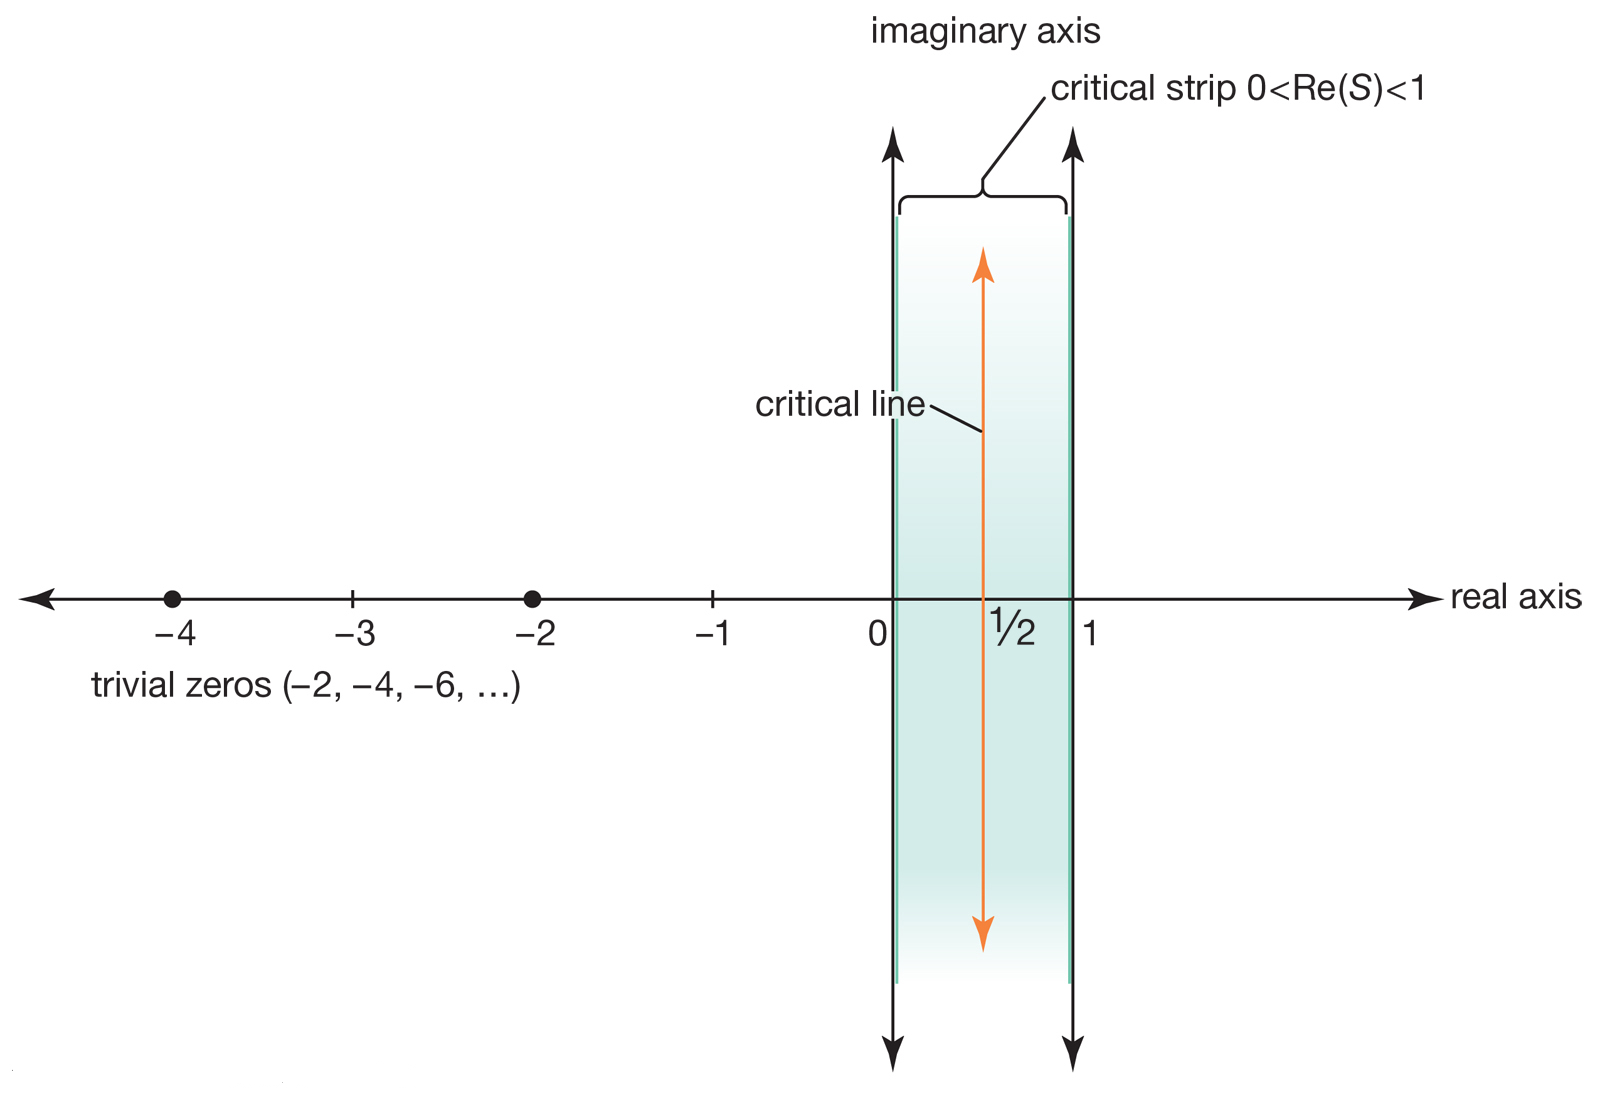
\includegraphics[scale=0.33]{zeta_funkcija.png}
\caption{Netrivialne ničle Riemannove zeta funkcije ležijo na pasu $\{s; 0<\re(s)<1\}$. Vir slike je~\cite{britannica}.}
\end{center}
\end{figure}

\begin{izrek}[Riemannova hipoteza]
Vse netrivialne ničle Riemannove zeta funkcije ležijo na premici $s=\{\frac{1}{2}+it; t \in \mathbb{R} \}$.
\end{izrek}

%%%%%%%%%%%%%%%%%%%%%%%%%%%%%%%%%%%%%%%%%%%%%%%%%%%%%%%%%%%%%%%%%%%%%%%%%%%% 
% Ekvivalentne trditve
\subsection{Ekvivalentne trditve}

Obstaja več ekvivalentnih formulacij Riemannove hipoteze. Dokazali bomo eno izmed njih, ki vključuje Fareyevo zaporedje. Pred tem se spomnimo M\"obiusove funkcije $\mu$ -- srečali smo jo v definiciji~\ref{def:MobFun}. Z njo je povezana naslednja funkcija.

\begin{definicija}
Naj bo $n \in \mathbb{N}$. \emph{Mertensova\footnote{Franz Mertens, 20.\ 3.\ 1840--5.\ 3.\ 1927, poljski matematik.} funkcija} je definirana s predpisom
\begin{equation}
M(n)=\sum_{k\leq n}\mu(k).
\end{equation}
\end{definicija}

\begin{primer}
Izračunajmo vrednosti Mertensove funkcije za nekaj naravnih števil:

\( M(2) = \mu(1) + \mu(2) = 1 - 1 = 0, \)

\( M(3) = \mu(1) + \mu(2) + \mu(3) = 1 - 1 - 1 = -1, \)

\( M(6) = \mu(1) + \mu(2) + \mu(3) + \mu(4) + \mu(5) + \mu(6) = 1 - 1 - 1 + 0 - 1 + 1 = -1. \)
\end{primer}

Mertensova funkcija ni monotona, njena vrednost pa se v vsakem naslednjem naravnem številu spremeni kvečjemu za $\pm 1$. Za vsako naravno število $n$ velja $|M(n)| \leq n$.

Naslednjo trditev, ki jo bomo navedli brez izpeljave, je leta 1912 dokazal Littlewood\footnote{John Edensor Littlewood, 9.\ 6.\ 1885--6.\ 9.\ 1977, angleški matematik.}. Njeno bistvo je, da Riemannovo hipotezo lahko prevedemo na ekvivalentno trditev, ki opisuje rast Mertensove funkcije. 
Več podrobnosti o njej si bralec lahko prebere v \cite[poglavje 12.1]{zetafunction}.
%
Oglejmo si le idejo za formulacijo trditve.

Če faktorje v Eulerjevi produktni formuli pomnožimo, dobimo na polravnini $\{s; \re(s)>1\}$ izražavo $ \frac{1}{\zeta(s)} = \sum_{n=1}^{\infty} \frac{\mu(n)}{n^s} $. 
Po nekaj korakih pridemo do zveze $ \frac{1}{\zeta(s)} = s \int_{0}^{\infty} M(x) x^{-s-1}dx $. 
Mertensovo funkcijo tu razumemo kot definirano za vse nenegativne vrednosti: predpišemo $M(0)=0$, funkcija pa je konstantna, razen v naravnih številih $n$, kjer ima skok $\mu(n)$.
Ker za vse $x$ velja $ |M(x)| \leq x $, je na polravnini $\{s; \re(s)>1\}$ $ \lim_{x \to \infty} x^{-s}M(x) = 0$ in integral $ \int_{0}^{\infty} M(x) x^{-s-1}dx $ na tej polravnini konvergira.
Če obstaja tako pozitivno število $a$, da funkcija $M$ raste počasneje od funkcije $x \mapsto x^{a}$, potem zgornji integral konvergira na polravnini $\{s; \re(a-s)<0\} = \{s; \re(s)>a\}$.
To pomeni, da je funkcija $s \mapsto \zeta^{-1}(s) $ na tej polravnini analitična. 
Vendar obstajajo ničle funkcije $\zeta$ na premici $s = \{\frac{1}{2}+it; t \in \mathbb{R} \}$, torej ima na tej premici funkcija $\zeta^{-1}$ singularnosti.
Od tod sledi, da za poljuben $0<a<\frac{1}{2}$ ne velja $M(x) = o(x^{a})$.
Naslednja trditev pove, da velja celo več. Še prej pa vpeljimo nov pojem.

% notacija mali o
\begin{definicija}[Notacija mali o]
Funkcija $f$ pripada razredu $o \left(g(x) \right)$, če absolutna vrednost funkcije $f$ raste počasneje od funkcije $g$.
Natančneje, $f(x) = o \left(g(x) \right)$, če za vsak $\varepsilon>0$ obstaja vrednost $x_{0}$, da za poljuben $x \geq x_{0}$ velja $|f(x)| < \varepsilon \cdot g(x)$.
\end{definicija}

\begin{trditev}
Za vsak $\varepsilon>0$ velja \( M(n) = o(n^{1/2+\varepsilon}) \) natanko tedaj, ko velja Riemannova hipoteza.
\end{trditev}

Pred drugo ekvivalenco Riemannove hipoteze potrebujemo definicijo, ki sledi.

\begin{definicija}
Naj bosta $L(n)$ dolžina Fareyevega zaporedja reda $n$ in $r_{v}$ njegov $v$-ti element. Definiramo razliko
\begin{equation}
\delta_{v}= r_{v}-v/L(n).
\end{equation}
\end{definicija}

\begin{primer}
Vzemimo Fareyevo zaporedje reda $4$ in poglejmo nekaj razlik:

\(F_4 = \left \{\frac{0}{1}, \frac{1}{4}, \frac{1}{3}, \frac{1}{2}, \frac{2}{3}, \frac{3}{4}, \frac{1}{1} \right \}, \)

\( L(4) = 7, \)

\( \delta_{1}= \frac{0}{1} - \frac{1}{7} = -\frac{1}{7}, \)

\( \delta_{2}= \frac{1}{4} - \frac{2}{7} = -\frac{1}{28}, \)

\( \delta_{7}= \frac{1}{1} - \frac{7}{7} = 0. \)

Opazimo, da za poljuben $n$ velja $\delta_{L(n)}=0$.
\end{primer}

\begin{trditev}[Franel-Landau, 1924]
Za vsak $\varepsilon>0$ velja \( \sum_{v=1}^{L(n)}|\delta_{v}| = o(n^{1/2+\varepsilon}) \) natanko tedaj, ko velja Riemannova hipoteza.
\end{trditev}

Dokaz zgornje trditve izpustimo. V obliki, kot sta ga dokazala Franel in Landau leta 1924, se nahaja v viru~\cite{franel-landau}. Pač pa bomo v nadaljevanju dokazali povezavo med navedenima ekvivalentnima formulacijama Riemannove hipoteze, ki jo lahko združimo v izrek.

\begin{izrek}
\label{Izr:RH}
Naj bo $\varepsilon > 0$. \( \sum_{v=1}^{L(n)}|\delta_{v}| = o(n^{1/2+\varepsilon}) \) velja tedaj in le tedaj, ko velja \( M(n) = o(n^{1/2+\varepsilon}). \)
\end{izrek}

%%%%%%%%%%%%%%%%%%%%%%%%%%%%%%%%%%%%%%%%%%%%%%%%%%%%%%%%%%%%%%%%%%%%%%%%%%%%%%%% Fareyevo zaporedje in RH
\subsection{Fareyevo zaporedje in Riemannova hipoteza}

V tem razdelku bomo dokazali glavni izrek~\ref{Izr:RH}, ki Riemannovo hipotezo poveže s Fareyevim zaporedjem. Najprej bomo dokazali lemo, ki bo ključ do dokaza izreka.

\begin{trditev}[M\"obiusova inverzija]
Naj bosta vrsti $\sum_{n=1}^{\infty} f(nx)$ in $\sum_{n=1}^{\infty} g(nx)$ absolutno konvergentni. Tedaj velja
\begin{equation}
g(x) = \sum_{n=1}^{\infty} f(nx) \Longleftrightarrow f(x) = \sum_{n=1}^{\infty} \mu(n) g(nx).
\end{equation}
Formulo lahko zapišemo v ekvivalentni obliki
\begin{equation}
\label{Eq:MobInv}
g(x) = \sum_{n=1}^{\infty} f \left(\frac{x}{n} \right) \Longleftrightarrow f(x) = \sum_{n=1}^{\infty} \mu(n) g \left(\frac{x}{n} \right).
\end{equation}
%
\end{trditev}

Trditev navajamo brez izpeljave -- ta se nahaja v \cite[poglavje 10.9]{zetafunction}. M\"obiusovo inverzijo bomo namreč potrebovali le v enem koraku dokaza napovedane leme, kjer bomo uporabili ekvivalenco~\eqref{Eq:MobInv}.

\begin{lema}
\label{Lema:RiemFar}
Realna funkcija $f$ naj bo definirana na intervalu $[0,1]$. Naj bodo $r_{v}$ elementi Fareyevega zaporedja reda $n$, $r_{0}=0$ in $r_{L(n)}=1$\footnote{Zgolj zaradi preglednejšega zapisa bomo za potrebe dokaza v tem razdelku Fareyevo zaporedje $F_{n}$ opazovali od neničelnega člena dalje. Tako bo element $r_{v}$ zdaj predstavljal element $r_{v+1}$ v običajni notaciji, vrednost $L(n)$ pa se bo zmanjšala za $1$.}. Tedaj velja enakost\footnote{Vsota na desni strani je končna, saj je za $k>n$ vrednost $M(\frac{n}{k})=0$.}
\begin{equation}
\label{Eq:RiemFar1}
	\sum_{v=1}^{L(n)} f(r_v) = \sum_{k=1}^{\infty} \sum_{j=1}^{k} f \left(\frac{j}{k} \right) M \left(\frac{n}{k} \right).
\end{equation}
\end{lema}

\begin{dokaz}
Funkcijo $D: \mathbb{R} \to \{0,1\}$ definirajmo s predpisom
\begin{align}
\label{Eq:D(n)}
D(n) = \left\{
\begin{array}{rl}
	1 &,\ \textrm{če}\ n \geq 1 \\
	0 &,\ \textrm{če}\ n < 1
\end{array}.
\right.
\end{align}
Spomnimo se definicije Mertensove funkcije in upoštevajmo predpis~\eqref{Eq:D(n)}. Dobimo
\begin{align*}
M(n) = \sum_{x \leq n} \mu(x) = \sum_{x=1}^{\infty} \mu(x) D \left( \frac{n}{x} \right),
\end{align*}
M\"obiusova inverzija pa nam da ekvivalenco
\begin{align*}
M(n) = \sum_{x=1}^{\infty} \mu(x) D \left( \frac{n}{x} \right) \Longleftrightarrow
D(n) = \sum_{x=1}^{\infty} M \left( \frac{n}{x} \right).
\end{align*}
Naj bosta celi števili $p$ in $q$ tuji ter $0 < p \leq q \leq n$, z drugimi besedami, ulomek $\frac{p}{q}$ ustreza nekemu elementu $r_{v}$ Fareyevega zaporedja $F_{n}$.
Primerjali bomo koeficiente pri $f(\frac{p}{q})$ na levi in desni strani enakosti~\eqref{Eq:RiemFar1}.
Ker je $ f(\frac{p}{q}) = f(\frac{2p}{2q}) = f(\frac{3p}{3q}) = \cdots $, je koeficient pri $f(\frac{p}{q})$ na desni strani enak 
%
\begin{align*}
M \left(\frac{n}{q} \right) + M \left(\frac{n}{2q} \right) + M \left(\frac{n}{3q} \right) + \cdots &= \sum_{l=1}^{\infty} M \left(\frac{n}{ql} \right) \\
&= D \left(\frac{n}{q} \right) = \left\{
\begin{array}{rl}
	1 &,\ \textrm{če}\ n \geq q \\
	0 &,\ \textrm{če}\ n < q
\end{array}.
\right.
\end{align*}
%
To pa je ravno koeficient pri $f(r_{v})$ na levi strani. Lema zato res drži.
%
\end{dokaz}

%%%
% Dokaz implikacije v desno
\subsubsection{Dokaz implikacije v desno izreka~\ref{Izr:RH}}

Naj bo $\varepsilon > 0$. Naj bo $u \in [0,1]$ in definirajmo funkcijo $f(u) = e^{2\pi iu}$. Uporabimo lemo~\ref{Lema:RiemFar} in funkcijo vstavimo v enakost~\eqref{Eq:RiemFar1}; dobimo
\begin{equation}
\label{Eq:RiemFar2}
	\sum_{v=1}^{L(n)} e^{2\pi i r_{v}} = \sum_{k=1}^{\infty} \sum_{j=1}^{k} e^{2\pi i \frac{j}{k}} M \left(\frac{n}{k} \right).
\end{equation}
Vemo, da je $\sum_{j=1}^{k} e^{2\pi i \frac{j}{k}} = 0$ za $k \geq 2$, za $k=1$ pa se vsota poenostavi v $e^{2\pi i} = 1$.
Enakost~\eqref{Eq:RiemFar2} zato prepišemo v 
\[ M(n) = \sum_{v=1}^{L(n)} e^{2\pi i r_{v}} = \sum_{v=1}^{L(n)} e^{2\pi i \left(\frac{v}{L(n)} + \delta_{v} \right)} 
	   = \sum_{v=1}^{L(n)} e^{ \frac{2\pi i v}{L(n)} } \left(e^{2\pi i \delta_{v}} - 1 \right) + \sum_{v=1}^{L(n)} e^{ \frac{2\pi iv}{L(n)} }. \]
Ker je $L(n) > 1$, je zadnji sumand enak $0$. Sedaj ocenimo absolutno vrednost zgornjega izraza:
\begin{align*} 
|M(n)| &\leq \sum_{v=1}^{L(n)} \left|e^{ \frac{2\pi i v}{L(n)} } \right| \left|e^{2\pi i \delta_{v}} - 1 \right| 
	= \sum_{v=1}^{L(n)} \left|e^{2\pi i \delta_{v}} - 1 \right|
	= \sum_{v=1}^{L(n)} \left|e^{\pi i \delta_{v} } \right| \left|e^{\pi i \delta_{v}} - e^{-\pi i \delta_{v}}\right| \\
	&= 2 \sum_{v=1}^{L(n)} |\sin{(\pi \delta_{v})}| \leq 2 \sum_{v=1}^{L(n)} |\delta_{v}| \pi = 2 \pi \sum_{v=1}^{L(n)} |\delta_{v}| \\
	&< 2 \pi K_{1}(\varepsilon) n^{1/2 + \varepsilon} = K(\varepsilon) n^{1/2 + \varepsilon}.
\end{align*}
V zadnji neenakosti smo uporabili predpostavko $ \sum_{v=1}^{L(n)}|\delta_{v}| = o(n^{1/2+\varepsilon}) $, kar je ekvivalentno 
$ \sum_{v=1}^{L(n)}|\delta_{v}| < K_{1}(\varepsilon) n^{1/2+\varepsilon}$ za neko konstanto $K_{1}$, ki je odvisna od $\varepsilon$.
Od tod sledi, da je $M(n) = o(n^{1/2 + \varepsilon})$, kar smo želeli pokazati.

%%%
% Bernoullijevi polinomi
\subsubsection{Bernoullijevi polinomi}

Preden se lotimo dokazovanja obratne implikacije, potrebujemo nekaj novih pojmov. Navedli bomo le najpomembnejše rezultate, ki jih bomo v dokazu potrebovali. Izpeljave niso pretežke, vendar jih bomo tokrat izpustili, saj bi precej povečale obseg dela. Rezultati so povzeti po \cite[poglavje 6.2]{zetafunction}.

\begin{definicija}
Naj bo $n \in \mathbb{N} \cup \{0\}.$ \emph{$n$-ti Bernoullijev polinom} $B_{n}$ je polinom stopnje $n$, ki ustreza zvezi
\begin{equation}
\label{Eq:BernPol}
\int_{x}^{x+1} B_{n}(t) dt = x^{n}.
\end{equation}
\end{definicija}

\begin{primer}
Zapišimo nekaj Bernoullijevih polinomov najnižjih stopenj. Izračunamo jih tako, da zapišemo polinom $B_{n}(t) = a_{0} + a_{1}t + \cdots + a_{n}t^{n}$ in rekurzivno računamo koeficiente pri potencah $x$ v enakosti~\eqref{Eq:BernPol}:

\( B_{0}(x) = 1, \)

\( B_{1}(x) = x - \frac{1}{2}, \)

\( B_{2}(x) = x^2 - x + \frac{1}{6}, \)

\( B_{3}(x) = x^3 - \frac{3}{2} x^2 + \frac{1}{2} x. \)
\end{primer}

\begin{definicija}
Naj bo $B_{n}$ $n$-ti Bernoullijev polinom. Pripadajoča funkcija $ \bar{B_{n}} $ je definirana kot $ \bar{B_{n}}(x) = B_{n}(x - \lfloor x \rfloor). $
\end{definicija}

\begin{opomba}
Iz definicije sledi, da je $ \bar{B_{n}} $ periodična funkcija s periodo $1$.
\end{opomba}

\begin{primer}
Funkcijo $ \bar{B_{1}}(x) = x - \lfloor x \rfloor - \frac{1}{2} $ bomo potrebovali v dokazu.
\end{primer}

\begin{figure}[h!]
\begin{center}
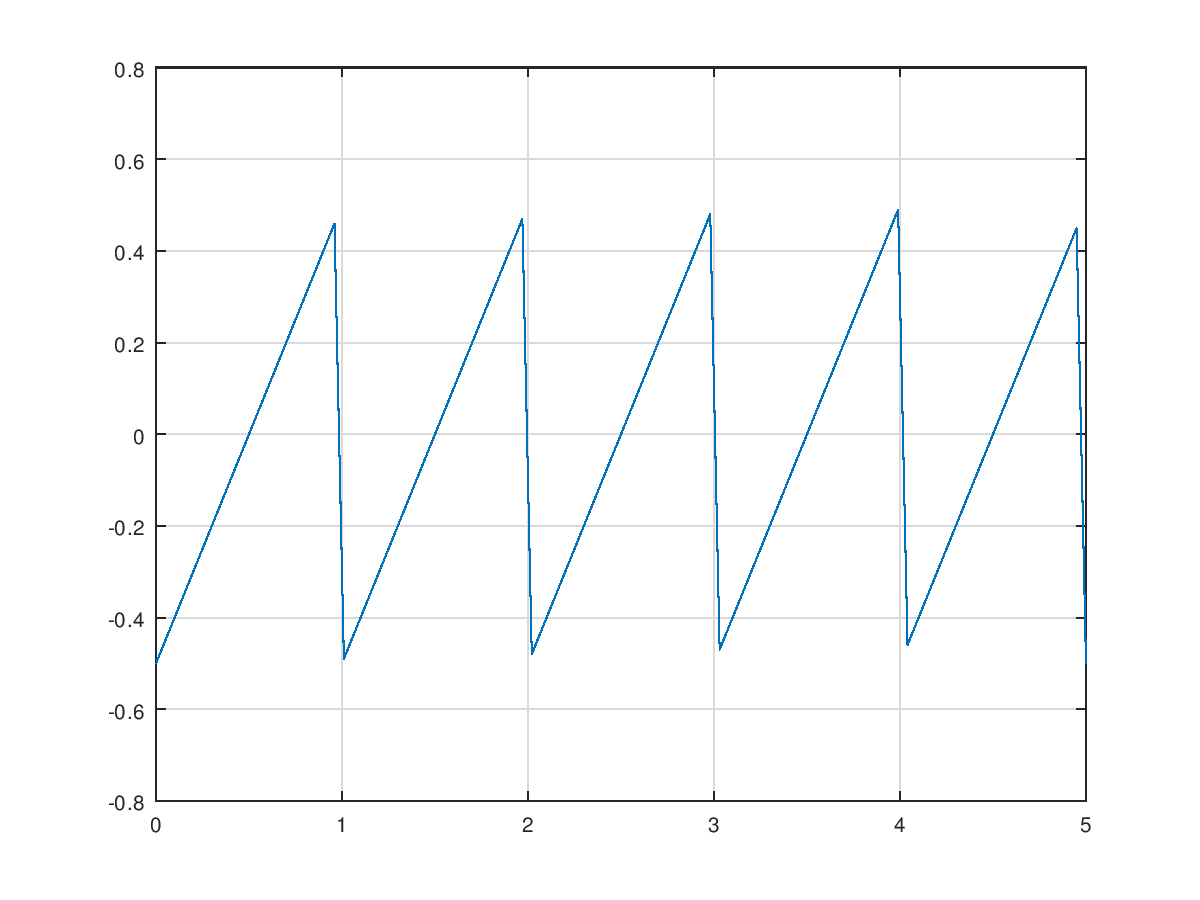
\includegraphics[scale=0.45]{bernoulli.png}
\caption{Graf funkcije $ \bar{B_{1}}(x) = x - \lfloor x \rfloor - \frac{1}{2} $.}
\end{center}
\end{figure}

\begin{trditev}
Naj bo $k \in \mathbb{N}$. Tedaj je
\begin{equation}
\label{Eq:B_{n}(ku)}
B_{n}(ku) = k^{n-1} \left ( B_{n}(u) + B_{n} \left( u + \frac{1}{k} \right) + \cdots + B_{n} \left( u + \frac{k-1}{k} \right) \right).
\end{equation}
\end{trditev}

\begin{dokaz}
Dokaz za $k=2$ se nahaja v \cite[poglavje 6.2, str.~102--103]{zetafunction}. Za splošen $k$ je dokaz analogen.
\end{dokaz}

%%%
% Dokaz implikacije v levo
\subsubsection{Dokaz implikacije v levo izreka~\ref{Izr:RH}}

Spomnimo se funkcije $ \bar{B_{1}}(x) = x - \lfloor x \rfloor - \frac{1}{2} $ in enačbe~\eqref{Eq:B_{n}(ku)}. Izberimo $n=1$. Funkcija $\bar{B_{1}}$ je periodična s periodo $1$, zato je za $x=ku$ dovolj obravnavati vrednosti $0 \leq u \leq \frac{1}{k}$. Za te vrednosti pa se $\bar{B_{1}}$ ujema s funkcijo $B_{1}$. Enačba~\eqref{Eq:B_{n}(ku)} zato dobi obliko
\begin{align}
\label{Eq:bar{B_{1}}(ku)}
\bar{B_{1}}(ku) &= \bar{B_{1}}(u) + \bar{B_{1}} \left( u + \frac{1}{k} \right) + \cdots + \bar{B_{1}} \left( u + \frac{k-1}{k} \right) \nonumber \\
			&= \bar{B_{1}} \left( u + \frac{1}{k} \right) + \bar{B_{1}} \left( u + \frac{2}{k} \right) + \cdots + \bar{B_{1}} \left( u + 1 \right).
\end{align}
%
Ključni korak dokaza je, da v enakost iz leme~\ref{Lema:RiemFar} vstavimo funkcijo $ \bar{B_{1}}$, pri čemer uporabimo zvezo~\eqref{Eq:bar{B_{1}}(ku)}. Označimo
\begin{align}
G(u) &= \sum_{v=1}^{L(n)} \bar{B_{1}}(u+r_v) = \sum_{k=1}^{\infty} \sum_{j=1}^{k} \bar{B_{1}} \left(u + \frac{j}{k} \right) M \left(\frac{n}{k} \right)
	= \sum_{k=1}^{\infty} \bar{B_{1}}(ku) M \left(\frac{n}{k} \right),
\end{align}
kar nam da dva izraza za funkcijo $G$. Izračunali bomo integral 
\begin{equation}
I = \int_{0}^1 G(u)^2 du.
\end{equation}

% 1. primer
\underline{1.~primer:} $G(u) = \sum_{v=1}^{L(n)} \bar{B_{1}}(u+r_v)$.
Oglejmo si, kakšna je funkcija $G$. Razpišimo zgornjo zvezo v
\begin{align}
G(u) &= \sum_{v=1}^{L(n)} \bar{B_{1}}(u+r_v) = \sum_{v=1}^{L(n)} \left(u+r_v - \lfloor u+r_v \rfloor - \frac{1}{2} \right) \nonumber \\
       &= L(n)u + \sum_{v=1}^{L(n)}r_v - \sum_{v=1}^{L(n)} \lfloor u+r_v \rfloor - \frac{L(n)}{2}
\end{align}
in opazujmo člen s spodnjim celim delom. Ker so členi Fareyevega zaporedja razen $r_{L(n)}=1$ simetrično razporejeni okrog vrednosti $\frac{1}{2}$, lahko zapišemo $\sum_{v=1}^{L(n)} \lfloor u+r_v \rfloor = \sum_{v=1}^{L(n)} \lfloor u+1-r_v \rfloor$. Za $u\in[0,1]$ zavzame $\lfloor u+1-r_v \rfloor$ le celi števili $0$ in $1$; slednje je le v primeru, ko je $u=r_{v}$. Zato je 
\[
\sum_{v=1}^{L(n)} \lfloor u+1-r_v \rfloor = \left\{
\begin{array}{rl}
	1 &,\ \textrm{če}\ u = r_{v}\\
	0 &,\ \textrm{sicer}
\end{array},
\right.
\]
kar pomeni, da ima funkcija $G$, evaluirana v elementih Fareyevega zaporedja, skok za $-1$. Med Fareyevima sosedoma, torej na intervalu $[r_{v-1},r_{v}]$, je $G$ linearna funkcija spremenljivke $u$ s koeficientom $L(n)$.
Zaradi simetrije členov Fareyevega zaporedja velja še $\sum_{v=1}^{L(n)-1} \bar{B_{1}}(r_v) = 0$. Od tod izračunamo desno limito funkcije $G$ v točki $0$,
\[ \lim_{u \to 0} G(u) = \lim_{u \to 0} \bar{B_{1}}(u+1) = -\frac{1}{2}. \]
Funkcija $G$ se zato na intervalu $[r_{v},r_{v+1}]$ izraža s predpisom
\[ G(u) = L(n)u - v - \frac{1}{2}. \]
%
Izrazimo še 
\[ L(n)r_{v} = L(n) \left( r_{v}-\frac{v}{L(n)}+\frac{v}{L(n)} \right) = L(n) \delta_{v} + v, \]
\begin{align*}
L(n)r_{v}-v+\frac{1}{2} &= L(n) \delta_{v} + \frac{1}{2}, \\
L(n)r_{v-1}-v+\frac{1}{2} &= L(n) \delta_{v-1} - \frac{1}{2}.
\end{align*}
%
Sedaj lahko izračunamo integral 
\begin{align}
\label{Eq:I1}
I &= \sum_{v=1}^{L(n)} \int_{r_{v-1}}^{r_{v}} \left( L(n)u-v-\frac{1}{2}+1 \right)^2 du \nonumber \\
  &= \sum_{v=1}^{L(n)} \frac{(L(n)u-v+\frac{1}{2})^3}{3L(n)} \bigg \arrowvert_{r_{v-1}}^{r_{v}} \nonumber \\
  &= \frac{1}{3L(n)} \sum_{v=1}^{L(n)} \left( \left(L(n) \delta_{v} + \frac{1}{2} \right)^3 - \left(L(n) \delta_{v-1} - \frac{1}{2} \right)^3 \right) \nonumber \\
  &= \frac{1}{3L(n)} \sum_{v=1}^{L(n)} \left( \left(L(n) \delta_{v} + \frac{1}{2} \right)^3 - \left(L(n) \delta_{v} - \frac{1}{2} \right)^3 \right) \nonumber \\
  &= \frac{1}{3L(n)} \sum_{v=1}^{L(n)} \left(3 \left(L(n) \delta_{v} \right)^2 + \frac{1}{4} \right) \nonumber \\
  &= L(n) \sum_{v=1}^{L(n)} \delta_{v}^2 + \frac{1}{12L(n)} L(n) \nonumber \\
  &= L(n) \sum_{v=1}^{L(n)} \delta_{v}^2 + \frac{1}{12}.
\end{align}
Zaradi privzetka, da je $r_{0}=0$ in $r_{L(n)}=1$, prva enakost res drži.
V četrti enakosti smo upoštevali, da je $\delta_{L(n)}=0$ in $L(n) \delta_{0}-\frac{1}{2} = L(n) \delta_{L(n)}-\frac{1}{2}.$

% 2. primer
\underline{2.~primer:} $G(u) = \sum_{k=1}^{\infty} \bar{B_{1}}(ku) M \left(\frac{n}{k} \right)$.
Računajmo integral
\begin{align}
\label{Eq:I_{ab}}
I &= \int_{0}^1 \left( \sum_{k=1}^{\infty} \bar{B_{1}}(ku) M \left(\frac{n}{k} \right) \right)^2 du \nonumber \\
  &= \int_{0}^1 \sum_{a=1}^{\infty} \sum_{b=1}^{\infty} \bar{B_{1}}(au) \bar{B_{1}}(bu) M \left(\frac{n}{a} \right) M \left(\frac{n}{b} \right) du \nonumber \\
  &= \sum_{a=1}^{\infty} \sum_{b=1}^{\infty} M \left(\frac{n}{a} \right) M \left(\frac{n}{b} \right) \int_{0}^1 \bar{B_{1}}(au) \bar{B_{1}}(bu) du,
\end{align}
% 
in označimo $I_{ab} = \int_{0}^1 \bar{B_{1}}(au) \bar{B_{1}}(bu) du.$ Vrednost tega integrala bomo izračunali v treh korakih.

Naj bo $b=1$. Tedaj je
\begin{align}
I_{a1} &= \int_{0}^1 \bar{B_{1}}(au) \bar{B_{1}}(u) du
	= \frac{1}{a} \int_{0}^a \bar{B_{1}}(v) \bar{B_{1}} \left(\frac{v}{a} \right) dv \nonumber \\
	&= \frac{1}{a} \sum_{k=0}^{a-1} \int_{0}^1 \bar{B_{1}}(k+t) \bar{B_{1}} \left(\frac{k}{a}+\frac{t}{a} \right) dt \nonumber \\
	&= \frac{1}{a} \int_{0}^1 \bar{B_{1}}(t) \bar{B_{1}} \left(a\frac{t}{a} \right) dt
	= \frac{1}{a} \int_{0}^1 \left( t-\frac{1}{2} \right)^2 dt \nonumber \\
	&= \frac{1}{3a} \left( t-\frac{1}{2} \right)^3 \bigg \arrowvert_{0}^{1}
	= \frac{1}{12a}.
\end{align}
V integrala smo zaporedoma uvedli novi spremenljivki $v=au$ in $v=k+t$. Nato smo upoštevali periodičnost funkcije $\bar{B_{1}}$ in zvezo \eqref{Eq:bar{B_{1}}(ku)}, ter uporabili dejstvo, da na intervalu $[0,1]$ velja $\bar{B_{1}}(t) = t-\frac{1}{2}$.

Oglejmo si primer, ko sta $a$ in $b$ tuji si števili. Računamo
\begin{align}
I_{ab} &= \int_{0}^1 \bar{B_{1}}(au) \bar{B_{1}}(bu) du
	= \frac{1}{a} \int_{0}^a \bar{B_{1}}(v) \bar{B_{1}} \left(\frac{bv}{a} \right) dv \nonumber \\
	&= \frac{1}{a} \sum_{k=0}^{a-1} \int_{0}^1 \bar{B_{1}}(k+t) \bar{B_{1}} \left(\frac{bk}{a}+\frac{bt}{a} \right) dt \nonumber \\
	&= \frac{1}{a} \int_{0}^1 \bar{B_{1}}(t) \bar{B_{1}} \left(a\frac{bt}{a} \right) dt
	= \frac{1}{a} I_{1b} 
	= \frac{1}{12ab}.
\end{align}
V zadnji vrstici smo upoštevali, da vrednosti $\frac{bk}{a}$ za $k \in \{0,1, \ldots, {a-1} \}$ pretečejo vse vrednosti iz množice $\{0, \frac{1}{a}, \ldots, \frac{a-1}{a}\}$.

Naj bo sedaj $c$ največji skupni delitelj števil $a$ in $b$. Zapišimo $a = c \alpha$ in $b = c \beta$ (seveda sta števili $\alpha$ in $\beta$ tuji). Velja
\begin{align}
I_{ab} &= \int_{0}^1 \bar{B_{1}}(c \alpha u) \bar{B_{1}}(c \beta u) du
	= \frac{1}{c} \int_{0}^c \bar{B_{1}}(\alpha t) \bar{B_{1}}(\beta t) dt \nonumber \\
	&= I_{\alpha \beta}
	= \frac{1}{12 \alpha \beta}
	= \frac{c^2}{12ab}.
\end{align}
V prvem integralu smo uvedli novo spremenljivko $t=cu$, nato pa upoštevali račun
\begin{align*}
\int_{k}^{k+1} \bar{B_{1}}(\alpha t) \bar{B_{1}}(\beta t) dt &= \int_{0}^{1} \bar{B_{1}}(\alpha s + \alpha k) \bar{B_{1}}(\beta s + \beta k) ds \\
 	&= \int_{0}^{1} \bar{B_{1}}(\alpha s) \bar{B_{1}}(\beta s) ds = I_{\alpha \beta}.
\end{align*}
%
Izračunano vrednost integrala $I_{ab}$ vstavimo v enakost \eqref{Eq:I_{ab}} in dobimo
\begin{equation}
\label{Eq:I2}
I = \sum_{a=1}^{\infty} \sum_{b=1}^{\infty} M \left(\frac{n}{a} \right) M \left(\frac{n}{b} \right) \frac{c^2}{12ab},
\end{equation}
kjer je $c$ največji skupni delitelj $a$ in $b$.

% Ocena in uporaba predpostavke
Naj bo $\varepsilon>0$. Predpostavljamo, da je $M(n) = o(n^{1/2+\varepsilon})$, kar pomeni, da obstaja taka konstanta $C$, odvisna od $\varepsilon$, da za poljubno velik $n$ velja $ |M(n)| < C(\varepsilon) n^{1/2+\varepsilon}$. Če to uporabimo v enačbi~\eqref{Eq:I2}, dobimo
\begin{align}
|I| &< \sum_{a=1}^{\infty} \sum_{b=1}^{\infty} C(\varepsilon)^2 \left( \frac{n}{a} \right)^{1/2+\varepsilon} \left( \frac{n}{b} \right)^{1/2+\varepsilon} \frac{c^2}{12ab} \nonumber \\
  &= n^{1+2\varepsilon} \frac{C(\varepsilon)^2}{12} \sum_{a=1}^{\infty} \sum_{b=1}^{\infty} \frac{c^2}{a^{3/2+\varepsilon} b^{3/2+\varepsilon}} \nonumber \\
  &= n^{1+2\varepsilon} \frac{C(\varepsilon)^2}{12} \sum_{a=1}^{\infty} \sum_{b=1}^{\infty} \frac{c^2}{\alpha^{3/2+\varepsilon} \beta^{3/2+\varepsilon} c^{3+2\varepsilon}} \nonumber \\
  &< n^{1+2\varepsilon} K_{1}(\varepsilon) \sum_{\alpha=1}^{\infty} \sum_{\beta=1}^{\infty} \sum_{c=1}^{\infty} \frac{1}{\alpha^{3/2} \beta^{3/2} c^{1+2\varepsilon}} \nonumber \\
  &= K_{2}(\varepsilon) n^{1+2\varepsilon}.
\end{align}
V zadnji neenakosti smo vsoto po tujih si številih $\alpha$ in $\beta$ zamenjali z vsoto po vseh naravnih številih $\alpha$ in $\beta$.

Sedaj se vrnimo k enakosti~\eqref{Eq:I1}, upoštevajmo, da je $|I| = I$, kar implicira
\[ I = L(n) \sum_{v=1}^{L(n)} \delta_{v}^2 + \frac{1}{12} < K_{2}(\varepsilon) n^{1+2\varepsilon}, \]
od koder sledi
\[ \sum_{v=1}^{L(n)} \delta_{v}^2 < K_{3}(\varepsilon) n^{1+2\varepsilon}. \]
Cauchy-Schwarzova neenakost nam da končno oceno
\begin{align*}
\sum_{v=1}^{L(n)} |\delta_{v}| &= \left| \sum_{v=1}^{L(n)} (\pm1)\delta_{v} \right|
	\leq \sqrt{\sum_{v=1}^{L(n)} (\pm1)^2}  \sqrt{\sum_{v=1}^{L(n)} \delta_{v}^2} 
	= L(n)^{1/2} \sqrt{\sum_{v=1}^{L(n)} \delta_{v}^2}
	< K(\varepsilon) n^{1/2+\varepsilon},
\end{align*}
kar dokazuje obratno implikacijo.

%
%%%%%%%%%%%%%%%%%%%%%%%%%%%%%%%%%%%%%%%%%%%%%%%%%%%%%%%%%%%%%%%%%%%%%%%%%%%%%%%%%%%%%%%%%%%%%%%%%%%%%%%%%%%%%%%%%%%%%%%%%%%%%%%%%%%%%%%%%%%%%%%%%%

\section*{Slovar strokovnih izrazov}

\geslo{Bernoulli}{\textbf{$\sim$ number} Bernoullijevo število; \textbf{$\sim$ polynomial} Bernoullijev polinom}
\geslo{Euler product formula}{Eulerjeva produktna formula -- povezuje Riemannovo zeta funkcijo s praštevili}
\geslo{Farey neighbour}{Fareyev sosed -- Fareyeva soseda sta sosednja elementa Fareyevega zaporedja}
\geslo{Ford neighbour}{Fordov sosed -- Fordova soseda sta tangentna Fordova kroga}
\geslo{group action}{delovanje grupe -- delovanje grupe G na množico M je homomorfizem iz grupe G v grupo permutacij množice M}
\geslo{little-o notation}{notacija mali o -- funkcija $f$ pripada razredu $o \left(g(x) \right)$, če absolutna vrednost funkcije $f$ raste počasneje od funkcije $g$}
\geslo{mediant}{medianta; \textbf{$\sim$ property} lastnost mediante -- lastnost mediante velja za Fareyevo zaporedje in Fordove kroge}
\geslo{Mertens function}{Mertensova funkcija}
\geslo{M\"obius function}{M\"obiusova funkcija}
\geslo{Riemann zeta function}{Riemannova zeta funkcija -- Riemannova hipoteza govori o ničlah te funkcije}

%%%%%%%%%%%%%%%%%%%%%%%%%%%%%%%%%%%%%%%%%%%%%%%%%%%%%%%%%%%%%%%%%%%%%%%%%%%%%%%%%%%%%%%%%%%%%%%%%%%%%%%%%%%%%%%%%%%%%%%%%%%%%%%%%%%%%%%%%%%%%%%%%%%%%%%%%%%%%%
% seznam uporabljene literature
\begin{thebibliography}{99}

\bibitem{fareyproject} J.~Ainsworth, M.~Dawson, J.~Pianta in J.~Warwick, \emph{The Farey sequence}, diplomsko delo, School of Mathematics, University of Edinburgh, 2012; dostopno tudi na \url{https://www.maths.ed.ac.uk/~v1ranick/fareyproject.pdf}.

\bibitem{zetafunction} H.~M.~Edwards, \emph{Riemann's zeta function}, Academic Press, Inc., New York, 1974.

\bibitem{ford} L.~R.~Ford, \emph{Fractions}, The American Mathematical Monthly, \textbf{45}, 1938, str.\ 586--601; dostopno tudi na \url{https://www.maths.ed.ac.uk/~v1ranick/papers/ford.pdf}.

\bibitem{franel-landau} J.~Franel in E.~Landau, \emph{Les suites de Farey et le probl\`eme des nombres premiers}, G\"ottinger Nachr., 1924, str.\ 198--206.

\bibitem{motifofmath} S.~B.~Guthery, \emph{A motif of mathematics}, Docent Press, Boston, 2011; dostopno tudi na \url{https://www.maths.ed.ac.uk/~v1ranick/papers/farey.pdf}.

\bibitem{hardy} G.~H.~Hardy in E.~M.~Wright, \emph{An introduction to the theory of numbers}, 4th ed., Oxford University Press, Oxford, 1960.

\bibitem{britannica} W.~L.~Hosch, \emph{Riemann hypothesis}, [ogled 8.~8.~2019], dostopno na \url{https://www.britannica.com/science/Riemann-hypothesis}.

\bibitem{bernoulli} P.~Sebah in X.~Gourdon, \emph{Introduction on Bernoulli's numbers}, verzija 12.~6.~2002, [ogled 20.~7.~2019], dostopno na \url{http://math.ucr.edu/~res/math153/s12/bernoulli-numbers.pdf}.

\bibitem{riemannHyp} J.~Veisdal, \emph{The Riemann hypothesis, explained}, verzija 21.~8.~2016, [ogled 30.~4.~2019], dostopno na \url{https://medium.com/cantors-paradise/the-riemann-hypothesis-explained-fa01c1f75d3f}.

\end{thebibliography}

\end{document}

